% !Mode:: "TeX:DE:UTF-8:Main"
% -*- mode: TeX -*- -*- coding: UTF-8 -*-
\listfiles
\def\UFcurrentpackage{chessboard}
\def\UFcurrentversion{1.8}
%$Date$$Version$


\RequirePackage{fix-cm}

\documentclass[pagesize,parskip=half-,fontsize=12pt]{scrartcl}
\usepackage[utf8]{inputenc}

%% chessboard specific commands
\usepackage[LSB1,LSB2, LSB3,LSBC2,LSBC3,LSBC4,LSBC5, T1]{fontenc}
%\usepackage[skak-parse]{xskak}
\usepackage{xskak}
\usepackage{pifont}
\usepackage{eqparbox}

\newcommand\Chess[1][1cm]{\boardfont\fontsize{#1}{#1}\setboardfontsize{#1}\selectfont}
\newcommand\Plus{\raisebox{0.5ex}{\normalfont\fontsize{1.5ex}{1.5ex}\bfseries\,+\,}}
\newcommand\Equal{\raisebox{0.5ex}{\normalfont\fontsize{1.5ex}{1.5ex}\bfseries\,=\,}}

\makeatletter
\newcommand\Describesetkey[4]{\par\index{#1}%
 \colorbox{yellow!50}{\makebox[\dimexpr\textwidth-2\fboxsep\relax]{\ttfamily%
  \eqparbox{setkey}{#1=\meta{#2}}\hfill
  \eqparbox{setexample}{%
     \ifthenelse{\equal{#3}{}}%
     {#1}
     {#1={#3}}}\hfill
  \eqparbox{setdefault}{\hfill #4}}}\par\nobreak\@afterheading}


\newcommand\Describefillkey[4][]{\par\index{#2}%
\makebox[0pt][r]{\scriptsize #1\hspace{1em}}%
 \colorbox{green!25}{\makebox[\dimexpr\textwidth-2\fboxsep\relax]{\ttfamily%
    \eqparbox{fillkey}{#2=\meta{#3}}\hfill
    \eqparbox{fillexample}{%
     \ifthenelse{\equal{#4}{}}%
     {#2}
     {#2={#4}}}}}%
    \par\nobreak\@afterheading}



\makeatother

%\usepackage{filecontents} only needed after change of docu.sty
\usepackage{UF-chessboard-documentation}

%initialisation
\setchessboard{smallboard, showmover=false}



\begin{document}
\newchessgame
\title{\packagename{chessboard}: A package to print chessboards}
\author{Ulrike Fischer}
\maketitle

\begin{center}
\newchessgame
\setchessboard{shortenend=5pt,color=red,margin=false}%
\unitlength1pt
\newcommand\currentboard[1][]{%
 \begin{picture}(150,150)
 \put(10,10){\chessboard[#1]}
 \end{picture}}%
\begin{animateinline}[autoplay,loop]{1}%
\currentboard
\newframe
\hidemoves{1.e4}%
\currentboard[pgfstyle=straightmove,markmove=e2-e4,
              pgfstyle=border,markfields={e2,e4}]
\newframe
\hidemoves{1... e5}%
\currentboard[pgfstyle=straightmove,markmove=e7-e5,
              pgfstyle=border,markfields={e7,e5}]
\newframe
\hidemoves{2. Nf3}%
\currentboard[pgfstyle=knightmove,markmove=g1-f3,
              pgfstyle=border,markfields={g1,f3}]
\newframe
\hidemoves{2... Nc6}%
\currentboard[pgfstyle=knightmove,markmove=b8-c6,
             pgfstyle=border,markfields={b8,c6}]
\newframe
\hidemoves{3.Bb5}%
\currentboard[pgfstyle=straightmove,markmove=f1-b5,
              pgfstyle=border,markfields={f1,b5}]
\newframe
\hidemoves{3... a6}%
\currentboard[pgfstyle=straightmove,markmove=a7-a6,
              pgfstyle=border,markfields={a7,a6}]
\end{animateinline}
\end{center}



\tableofcontents
\section{Changes}
\minisec{Attention!} From version 1.5 on the documentation uses the
(new) package \packagename{xskak} instead of \packagename{skak}. The
most notable difference is that in some examples \cs{newchessgame}
instead of \cs{newgame} is used. But in most cases all examples
should work with \packagename{skak} alone too. The package
\packagename{xskak} adds quite a lot new keys to \cs{chessboard} to
show arbitrary positions from previously parsed games. Read its
documentation if you want to use them.


In version 1.3 I made a lot of changes. I tried to preserve the
behaviour of existing keys and commands. But is possible that older
documents will look different when processed with this version.

Notably two things can give problems: The value of the
\key{padding} key now affects much more objects (marks) in the pgf
pictures. So it could be necessary to reset the padding. And the
\key{applycolor} has changed its behaviour. It will now also affect
the foreground picture.

\begin{description}
\item[2019-06-23 (Version 1.8)] Uploaded the source of the documentation to ctan.
  No longer use \cs{arabic} internally, to avoid problems with packages redefining the command. (Issue \#1).

\item[2011-03-17 (Version 1.7)] Changed definition of the triangle mover
    style. It now uses \packagename{tikz} and no longer
    \packagename{amssymb}. \packagename{chessboard} no longer loads
    \packagename{amssymb} (it clashes with \packagename{xunicode}).

\item[2011-03-13 (Version 1.7)] Corrected a bug with spacing when the
    \packagename{amsart} is used.


\item[2008-11-27 (Version 1.6)] Corrected a bug in \key{getpiecelists}
(empty lists were undefined).


\item[2007-12-11 (Version 1.5)] Added the key \key{getpiecelists} to
retrieve the positions of pieces. Quite a lot new keys to show
arbitrary positions from previously parsed games are added by the
package \packagename{xskak}. Read its documentation if you want to
use them.

\item[2007-08-20 (Version 1.5)] Added curvemove-style to draw moves.
Corrected some bugs. Changed a lot internally to adapt the package to
\packagename{xskak.sty}.

\item[2007-07-03 (Version 1.4)] Rewrote the code that process the
keys saved globally (with \cs{chessboard}) and  in styles (with
\cs{storechessboardstyle}) to go around a problem due to a change in
\packagename{xkeyval 2.5}. Corrected some errors in the
documentation.
\item[2006-07-20 (Version 1.3)] Rearranged and rewrote the keys and commands for
the pgf-pictures. Now all styles and marks can be used in both
pictures. Added definitions for partial borders. Extended trim and
clip commands. \packagename{xifthen} is now required.
\item[2006-06-22] Added keys for fancy borders, added local commands for
the boardarea and the printarea. Disabled the option skaknew as it
not longer works in \chessfss.
\end{description}




\section{Introduction}
\minisec{What is does} \DescribeMacro{\chessboard} This package
offers a command \cs{chessboard}\keyoarg{} to print boards of chess
positions and similar games. It is intended to replace the
\cs{showboard} command of \skaksty which has some deficiencies:
\begin{itemize}
\item To print a special position one always has to type the
complete FEN.
\item It frames all boards with a  rule of 1pt -- which is okay
for a large board but doesn't look good on small boards.
\item It's difficult (up to impossible) to color some squares.
\item Even for simple markings like crosses or the mover \skaksty use
postscript. That makes it difficult to use pdf\LaTeX.
\item It's difficult to print partial boards.
\item It's difficult (up to impossible) to print boards with exotic
pieces e.g.\ fairy chess.
\item It's impossible to print boards with unusual dimension or unusual labels used by other games e.g.\
10\texttimes10 boards with numbers instead of characters.
\item The labels at the bottom changes the baseline which makes it
difficult to align boards.
\item Some commands e.g., \cs{notationoff} of  \skaksty redefines \cs{skakboard}, so it
is difficult to patch the command e.g.\ to get larger margins.
\end{itemize}


With \pchessboard you have now full control about size, content and
look of the board. I have tried to make \cs{chessboard} as flexible
as possible. So I added a lot of options to change values that
control the size, layout and filling of the board. In most cases you
can ignore them but being able to change them can come handy if you
need something unusual.

But I didn't tried to stretch flexibility too much. The main aim of
the package is to print chessboards easily, so e.g.\ the inputs use
the naming conventions of chess. That means that -- as the files are
numbered alphabetically -- the width of the board is restricted to 26
fields (27 with option \key{zero}). The board is build with
alternating black and white fields, changing to e.g.\ three colors
could be difficult. The pieces are named with simple ASCII-chars, so
the number of different pieces is restricted. (It is perhaps possible
to define piecenames consisting of two or more chars, and to use such
names by putting braces around the chars e.g.,
\verb+{KK}a3+.  A small test worked fine for me, but I wouldn't bet
that it really works everywhere.)

\minisec{What it doesn't} \Pchessboard doesn't offer commands to type
captions or titles or a list of the chessboards. There are no options
that control the placement of the board in the text flow, e.g. to
center it or to let it float. This is a design decision.
\cs{chessboard} prints only chessboards like \cs{includegraphics}
inserts only graphics.



\subsection{Bugs and errors}

I'm quite sure that they are bugs and errors in the package. I did
find some quite horrible while making the documentation and I'm sure
I overlooked some. E.g.\ I have a lot of doubts if spaces and braces
in keys saved in a style or with \cs{setchessboard} are handled
correctly in every case.

If you have questions ask them in the newsgroups
\nolinkurl{comp.text.tex} or
\nolinkurl{de.comp.text.tex}. I'm reading these groups regularly and
I'm much better in answering there than in answering e-mails.


If you find errors in this text  (this includes wrong english) or in
the package, you can write me a bugreport at
\nolinkurl{skak@nililand.de}. A bugreport should contain a complete \emph{minimal}
example and the log-file of the pdf\LaTeX\ run (this is the engine
that makes a pdf!).

Before sending a bug record check the following things:


\minisec{If you get mysterious error messages}
\begin{itemize}
\item  Check the commas in the \keylists.
\end{itemize}

\minisec{Missing or faulty pgf-decorations}
\begin{itemize}
\item Check if the borders or marks are hidden under other decorations or under board chars with solid fieldmasks.
\item Check if trimming is responsible: try the key \verb+trim=false+.
\item Check the state of the key \key{pgf}.
\item Try another previewer, zoom in and out, print the document.
\item Go through your log-file and search for chessboard warnings.
\end{itemize}


\subsection{Requirements}

\Pchessboard uses some primitives of e\TeX. It needs a recent version
of \chessfss (chess font selection), \packagename{xkeyval}
(\textit{key=value}-syntax) and \packagename{xifthen}. It also needs
the packages \packagename{pgfcore}, \packagename{pgfbaseshapes} (from
pgf for the highlighting commands), \packagename{pst-node} (from
pstricks).


\subsection{Installation}
Run \filetype{chessboard.ins} through \LaTeX\ and then put the four
\filetype{.sty}-files somewhere where \LaTeX\ finds them.
\path{<texmf>/tex/latex/chessboard/} is a good place. Update the
filename database.

\subsection{Robustness: using \texorpdfstring{\cs{chessboard}}{\textbackslash chessboard} in moving arguments}
I have used \cs{chessboard} in tabulars and in moving arguments. It
seems to work fine, so I would say the command is quite robust.

Putting chessboards in the table of contents or the header will in
most case not look very good, so it is sensible to avoid it with
\lstinline+\section[short text]{\chessboard Title}+.
But if you want to do some advices:
\begin{itemize}
\item
Boards in the title and in the table of contents are built at different times during the run, when perhaps
different options and different games are active, so they can look
different if you are not careful.
\item You can't put boards in the bookmarks of a pdf, use
\verb+\texorpdfstring+ from \packagename{hyperref} to provide a
replacement.
\item Some pagestyles puts a command to uppercase around the header.
This affects keys in the optional argument of \cs{chessboard} and
will give error messages about undefined keys. Try to surround the
\cs{chessboard} command with \cs{lowercase}\verb+{...}+.
\end{itemize}



\subsection{Setting the options}

\Pchessboard use the keyval syntax \meta{key}\texttt{=}\meta{value}.

It differs in some respects to other packages with keyval syntax:
\mynobreakpar
\begin{itemize}
\item
There are really \emph{very} much keys.
\item
Some keys don't set properties of a board (like a width) but
\emph{do} things like drawing.
\item
The order of the keys can matter.
\item
Some effects are achieved by using two or more keys after one other.
\end{itemize}

There are keys that need a certain type of argument, e.g.\ a length
or a list of fields.  There are boolean keys that accept only the
values \texttt{=true} and \texttt{=false} where the value
\texttt{=true} can always be omitted. And at last there are keys
that works as \emph{commands}, you can use whatever argument you want
or leave it blank. Don't confound this commands with boolean keys.
E.g.\
\texttt{clearboard}, \texttt{clearboard=hallo} and even
\texttt{clearboard=false} will always clear the board.


I'm struggling permanently with the naming of the keys. Giving them
names that are not to long, but descriptive and a bit systematic
isn't easy. Also it isn't easy to decide if a special effect should
be achieve with one key (which gives a short input) or with a
combination of keys (with is more flexible as it can be used to
implement similar effects but gives longer input). While the package
evolved I sometimes tumbled in problems and inconsistencies of the
current naming scheme and had to reconsider my decisions and
implemented better names or new key combinations. I didn't delete or
disable older, now perhaps obsolate keys in any case, as I wanted to
avoid that older documents breaks.  I also sometimes add a key that
is simply a copy of an existing key only to get a more consistent
naming. So ist quite possible that you can get the same result with
different key combination. For a lot of things there isn't one
correct way -- you can choose the one which suits you more.


It's easy to make mistakes when using a lot of keys. So if you get
mysterious errors check that you don't have forgot a comma between
the keys, that you put braces around lists used as value, that you
didn't use a backslash before a key, that you didn't used a list of
fields when a list of pieces is requested.


\DescribeMacro{\setchessboard} You can set an option either for one
board by using the optional argument of \cs{chessboard} or by using
\cs{setchessboard}\keymarg{} which sets the keys for all following
boards in the same environment/group.

\begin{LTXexample}
Default setting in this Dokumentation:
\setchessboard{
      smallboard,
      showmover=false}
\newchessgame
\chessboard
\end{LTXexample}

Even if they share the same name, keys used in the argument of
\cs{chessboard} are implementated differently than the keys used in
\cs{setchessboard}. They do different things: In the first case the
key gets «executed» while in the second case the \keyvalue pair is
only stored for later use. So it is quite possible that a key works
with \cs{chessboard} but fails because of a bug when used in
\cs{setchessboard} or vice-versa.


Values set by keys in the argument of \cs{chessboard} will if
appropriate overwrite the ones set by \cs{setchessboard}.

The keys belong roughly to two classes: There are the keys that set
one property of the board, e.g.\ the width of a rule or the size.
Such keys always have a default and only the last value set is used,
it overwrites all previous values. Internally I call such keys
«set-keys». In the second class there are keys that can be used more
than once, e.g.\ keys that add a piece or a mark or a color to the
board. I call such keys «fill-keys».\footnote{I did realize only
quite late that using keys not only to set some parameters but also
for the real content is a bit unusual. It is a bit as if one would
use keys for the items of a list or the lines of tabular or the code
in a listing -- in most cases quite a bad idea. But at my opinion it
works fine in this special case because a chessboard is a quite
restricted room with only 64 fields.}


The «set-keys» are always processed first. Inside the classes the
keys are processed in general from «left to right», so later keys can
overwrite values set by earlier keys. This is also true for values
hidden in a \key{style}.






For each «set-key» you will find in this documentation a box like
this:

\Describesetkey{zero}{true|false}{false, zero}{false}


It shows on the left the general description of the possible values,
in the middle one or more examples of correct input, and on the
right the default value.

For each «fill-key» you will find in this documentation a box like
this:

\Describefillkey{clearranks}{list of ranks}{8}

It shows on the left the general description of the possible values
and on the right one or more examples of correct input.



\subsection{Saving optionlists}

\Describefillkey{style}{name}{mystyle}

\DescribeMacro{\storechessboardstyle} With the
\cs{storechessboardstyle}\marg{name}\keymarg{} it is possible to
store a list of \keyvalue-pairs in a «style» and to use this style
instead of the keys themselves.

\begin{LTXexample}
\storechessboardstyle{10x10}{%
 maxfield=j10,
 clearboard,
 startfen=b9,
 restorefen=current,
 labelleftwidth=1.5ex}

\storechessboardstyle{red-yellow}{%
 boardfontencoding=LSBC3,
  whitepiececolor=red,
  blackpiececolor=yellow,
  setfontcolors}

\setchessboard{style=red-yellow}
\newchessgame
\chessboard

\chessboard[style=10x10]
\end{LTXexample}

\minisec{Attention} \cs{storechessboardstyle} and \cs{setchessboard}
only store the \keyvalue pair, they don't expand anything and they
don't do anything with them. So be careful when using commands that
could be redefined later:

\begin{LTXexample}
\def\mylist{Ke1, qe2, kf3}
\setchessboard{setpieces=\mylist}
\def\mylist{Ke1, ra1, ke3}
\chessboard
\end{LTXexample}





\subsection{Naming the board}

In chess the rows of the board are called \emph{ranks} and are
numbered from 1 to 8. The columns are called \emph{files} and are
«numbered» from a to h.\footnote{%
I have some difficulties to remember the english names, so I use the
following mnemonics:
\textbf{F}i\textbf{L}e = co\textbf{L}umn = \textbf{L}inie =
al\textbf{F}abet,
\textbf{R}ank = \textbf{R}ow = \textbf{R}eihe = numbe\textbf{R}ed}

\Pchessboard use this naming conventions for all inputs:
Every time \meta{field} is used in this documentation, you should
give a char from a--z followed by a number.


\subsection{Naming areas of the board}

Rectangular areas are normally described by giving the coordinates
of the left bottom corner and the right upper corner. But when using
the Forsyth Edwards Notation (FEN) chessboards are filled starting
from the left upper corner a8 and then going on to the right and
down to the right bottom corner -- like the normal typesetting
direction. So it is quite natural to use for FEN related areas this
corners. As it would be awkward to have two different ways to
describe areas, I decided to use the fen convention everywhere: Each
area has a
\emph{startfield}, the left upper corner, and a \emph{stopfield},
the right bottom corner. If some area related keys  don't seem to
work, check that you have used the correct corners!


An area can also be given as two fields separated by an hyphen. When
using this input you don't have to worry about the corners, the
package will sort them:\\
\meta{area}=\meta{a corner}-\meta{the opposite corner}.


\DescribeMacro{\printarea} \DescribeMacro{\board} \cs{chessboard}
sets at the start this two command to the current values of the
printarea and the total board as given by the keys \key{zero},
\key{maxfield} and \key{printarea}. You can use this commands in
later keys.


\subsection{FEN: Forsyth-Edwards Notation}\label{sec:FEN}

FEN describes a chess position. It consist of 6 fields, separated by
spaces. The first field represents the placement of the pieces on
the board. The second field represents the active color.  A lower
case «w» is used if White is to move; a lower case «b» is used if
Black is the active player. The third field represents castling
availability. The fourth field is the en passant target square. The
fifth field is a nonnegative integer representing the halfmove
clock. The sixth and last field is a positive integer that gives the
fullmove number.

In the first field the board contents are specified starting with
the eighth rank and ending with the first rank («in typesetting
direction» when the board has the standard orientation). For each
rank, the squares are specified from file a to file h. White pieces
are identified by uppercase piece letters («\texttt{PNBRQK}») and
black pieces are identified by lowercase  piece letters
(«\texttt{pnbrqk}»). Empty squares are represented by the digits one
through eight; the digit used represents the count of contiguous
empty squares along a rank. A solidus character «\texttt{/}» is used
to separate data of adjacent ranks.

\cs{chessboard} handles FEN-input but also only «FEN-like»-input. If
given a complete FEN \cs{chessboard} will store all fields in
commands and evaluate the first field to fill the board. But if they
are less than six fields, \cs{chessboard} will not complain but
simply fill up the missing fields with some default values.

In the first field there don't need to be exact 8 pieces in each rank
and exactly 8 rank descriptions. When there are more pieces than
needed, \cs{chessboard} will ignore them. When there are less pieces
than needed then \cs{chessboard} will leave the remaining fields in
this rank untouched.


The FEN can also be stored in a command. So all \cs{chessboard} will
accept all the following inputs as \meta{FEN}:

{\ttfamily
 rnbqkbnr/pppppppp/8/8/8/8/PPPPPPPP/RNBQKBNR w KQkq - 0 1\\
 rnbqkbnr/pppppppp/8/8/8/8/PPPPPPPP/RNBQKBNR \\
 8qK\\
 10 w - - 0 10}\\
 \verb+\myfen+

\subsection{The main parts of the board}
Each chessboard is build by printing three «layers» on top of each
other:

\minisec{1. The background layer}

This is a pgf-picture that lies under the board. It can be used for
background colors or fancy borders or other background decoration.
%Coloring or drawing something in this layers means adding a color
%command or pgf commands to the code of the picture. How to do this
%will be described in the section about decorating the background.

%\minisec{2. The (four) font layers}
\minisec{2. The main board layer}
This is the main part of the board. It lies above the background
picture. It uses only «normal» \LaTeX\ objects like rules and chars.
Labels, movers and figures are all build together in this layer.

\minisec{3. The mark layer}

This layer is again a pgf picture now over the board. It can be used
to draw crosses, arrows etc on the board.

The sections \ref{startmain} to \ref{stopmain} describe how to
manipulate the main layer. The section \ref{startpgf} describes
how to handle the pgf pictures.






\section{Setting the contents of the board}\label{startmain}

\subsection{The maximum number of fields}
\Describesetkey{maxfield}{field}{j10}{h8}%
Chessboards have 8\texttimes8 fields. So this is the default. If you
want another size you should declare a new right upper corner  with
\key{maxfield=}\meta{Field} e.g., \key{maxfield=j10} for a 10\texttimes10 board.
Don't use this key if you want only to print a partial board, there
is another key to achieve this. Use it to change the maximum size
of a board. All fields and areas you use in other arguments should lie inside this maximum size.

\begin{LTXexample}
\newchessgame
\chessboard[tinyboard,
            maxfield=f6]
\end{LTXexample}


\begin{LTXexample}
\newchessgame
\chessboard[tinyboard,
            maxfield=j10,
            labelleftwidth=2ex]
\end{LTXexample}

\Describesetkey{zero}{true|false}{false}{false}%
I was told that some games numbers the fields starting with 0. So I
added this option. When set to true the rank numbers start with 0 and
a file named Z is added left to the file a.

\begin{LTXexample}
\newchessgame
\chessboard[zero,
            labelbottomformat=\arabic{filelabel},
            addpieces={KZ0, QZ8}]
\end{LTXexample}


\subsection{Filling with \skaksty}
When \skaksty is loaded and there is a running game, \cs{chessboard}
will fill the board with the current position.

\begin{LTXexample}
\newchessgame
\mainline{1. e4 e5 2. Nf3 Nc6 3. Bb5 a6}
\chessboard
\end{LTXexample}

\subsection{Clearing}
\Describefillkey{clearboard}{arbitrary}{}
\Describefillkey{cleararea}{area}{a1-c3}
\Describefillkey{clearareas}{list of areas}{\{a1-c3,g7-h8\}}
\Describefillkey{clearfile}{file}{g}
\Describefillkey{clearfiles}{list of files}{\{g,h\}}
\Describefillkey{clearrank}{rank}{5}
\Describefillkey{clearranks}{list of ranks}{\{8,7\}}
\Describefillkey{clearfield}{field}{c6}
\Describefillkey{clearfields}{list of fields}{\{b5,c6\}}

You can't prevent that \cs{chessboard}  fills up the board with the
running game, so if you need an empty board, you should clear it --
either with the keys mentioned here, or by using one of the  keys
described later that clears the board before adding new pieces.

\begin{LTXexample}
\newchessgame
\mainline{1. e4 e5 2. Nf3 Nc6 3. Bb5 a6}
\def\ranklist{7 ,6 }
\def\cleararea{a1-b2}
\chessboard[clearfiles=g,
            clearranks=\ranklist,
            cleararea=\cleararea,
            clearfields={b5,c6}]
\end{LTXexample}


\subsection{Adding single pieces}

\Describefillkey{setpieces}{List of piece positions}{\{Ke4, Qe1, kd6\}}%
\Describefillkey{addpieces}{List of piece positions}{\{Ke4, Qe1, kd6\}}%

The \key{setpieces} first clears the board and then set the pieces,
the \key{addpieces} only set the new pieces but lets the existing
pieces undisturbed.

\begin{LTXexample}
\newchessgame
\mainline{1. e4 e5 2. Nf3 Nc6 3. Bb5 a6}
\def\piecelist{Ke1,Qd1 , Rg1}
\chessboard[setpieces={ra1, rh8, ke8},
            addpieces=\piecelist]
\end{LTXexample}

\Describefillkey{setwhite}{List of piece positions}{\{Ke4, Qe1, kd6\}}
\Describefillkey{addwhite}{List of piece positions}{\{Ke4, Qe1, kd6\}}
\Describefillkey{setblack}{List of piece positions}{\{Ke4, Qe1, kd6\}}
\Describefillkey{addblack}{List of piece positions}{\{Ke4, Qe1, kd6\}}

It is a bit cumbersome to have to be careful to use uppercase chars
for the white and lowercase chars for the black piece. With the keys
\key{setwhite}, \key{addwhite}, \key{setblack} and \key{addblack}
you can add white and black pieces
without caring about the cases. Like the keys for adding pieces, the
keys starting with \key{set} first clears the board, so if you don't
want to loose all the set pieces, you should use such a key only
once.

\begin{LTXexample}
\def\whitepieces{kc3, nc2, pa2, Pd4}
\chessboard[setwhite=\whitepieces,
            addblack={Kc8,bh7, pa7}]
\end{LTXexample}


\subsection{Adding FEN-positions}


\Describefillkey{setfen}{FEN}{\string\myfen, rnbqk/8/RNBQK}
\Describefillkey{addfen}{FEN}{\string\myfen, rnbqk/8/RNBQK}

With this keys you can add pieces to the board by given a FEN. The
\key{setfen} will clear the board, \key{addfen} will left pieces
outside the fields described by the FEN undisturbed.

\begin{LTXexample}
\newchessgame
\def\myfen{KK//KK}
\chessboard[addfen=\myfen]
\end{LTXexample}

\Describefillkey{startfen}{field}{b7}%

As a default \cs{chessboard} fills the board with a FEN-position
starting at the left upper corner. You can shift this start field
with the key \key{startfen}.

\begin{LTXexample}
\newchessgame
\def\myfen{KK//KK}
\chessboard[startfen=c7, addfen=KK//KK,
            startfen=f3, addfen=\myfen]
\end{LTXexample}


\Describefillkey{startfill}{field}{b7}
\Describefillkey{stopfill}{field}{f2}
\Describefillkey{fillarea}{area}{c2-d4}

With this keys you can restrict the part of the board that is filled
by a FEN. Only the pieces inside the fillarea are set.

\begin{LTXexample}
\newchessgame
\def\myfen{kqrb///KQRB}
\chessboard[setfen=\myfen, startfen=e4, fillarea=f2-g4, addfen=\myfen]
\end{LTXexample}

\subsection{Saving positions}
\Skaksty has the command \cs{storegame}\marg{name} that stores the
FEN of the current game in an internal command, and the command
\cs{savegame}\marg{name} that stores the FEN in a file
\marg{name}\filetype{.fen}

\Pchessboard defines similar keys. The key \key{storefen}=\meta{name}
stores the FEN in an internal command \emph{with the same name} as
used by \cs{storegame}\marg{name}. That means that you can exchange
the games stored by \skaksty and \pchessboard, but it also means that
\pchessboard can \emph{overwrite} games stored with \skaksty. So be
careful!

\medskip
\Describefillkey{storefen}{name}{game1}
\Describefillkey{savefen}{name of file}{game}

\key{storefen} saves the current position as FEN to a internal command.
\key{savefen} saves the current position as FEN to a file.

\medskip
\Describefillkey{startstore}{field}{b7}
\Describefillkey{stopstore}{field}{f2}
\Describefillkey{storearea}{area}{c2-d4}

With this keys you can restrict the area that is stored or saved. But
attention: \skaksty absolutly doesn't like «illegal» FENs that
doesn't describe a full 8\texttimes8 board.

\medskip
\Describefillkey{mover}{w|b}{w}
\Describefillkey{castling}{castling possibilies}{Kq}
\Describefillkey{enpassant}{field|-}{c4}
\Describefillkey{halfmove}{number}{14}
\Describefillkey{fullmove}{number}{20}

With this keys you can set the rest of the FEN-fields. Apart from
\key{mover} the values are only used if you save FENs. The values
are also set, if you use in the argument of a
\key{setfen} or \key{addfen} key complete FENs instead of only the position part.

\subsection{Getting the positions of pieces}

\Describefillkey{getpiecelists}{}{}

New in version 1.5 there is a key, that retrieves the position of the
pieces on the board. For each piece type there is a list called
\cs{cblist}\meta{piece}.\index{cblists=\verb!*+\cblist+\meta{piece}}.
The lists can be used everywhere where a list of fields is expected.
E.g. it is possible to use the lists to highlight all pawns (see
section \ref{sec:drawfields}).

Unlike almost all other commands of \packagename{chessboard} this
commands are saved globally. This makes it possible to use the lists
after the board:

\begin{LTXexample}
 \newchessgame
 \chessboard[getpiecelists]

 White pieces: \king\cblistK, \queen\cblistQ,
               \rook\cblistR, \bishop\cblistB,
               \knight\cblistN, \pawn\cblistP.

 Black pieces: \king\cblistk, \queen\cblistq,
               \rook\cblistr, \bishop\cblistb,
               \knight\cblistn, \pawn\cblistp.
\end{LTXexample}


\subsection{Using saved and stored games}

When you are using \skaksty, you can use the saved games to set the
start position of a game with the \skaksty-commands
\cs{restoregame}\marg{name} (restores the game stored with
\cs{storegame}) and \cs{loadgame}\marg{name} (loads the game saved
with \cs{savegame}). This only works if you have saved the position
of a normal 8\texttimes8-board!



\medskip
\Describefillkey{restorefen}{name}{game1}
\Describefillkey{loadfen}{name}{game}

You can also use the saved games to set positions on \cs{chessboard}.
\key{restorefen} will use games saved with \cs{storegame} and
\key{storefen}, \key{loadfen} will load games saved with
\cs{savegame} and \key{savefen}.




\begin{LTXexample}
\newchessgame
\def\gamename{rank7}
\chessboard[storearea=a7-h7, storefen=\gamename,
            startfen=a5, restorefen=rank7]
\end{LTXexample}
\begin{LTXexample}
\mainline{1. e4 e5}
\savegame{file} % to file.fen
\mainline{2. Nf3 Nf6}
\def\filename{file}
\chessboard[loadfen=\filename]
\end{LTXexample}

\subsection{Restoring the running game}

\cs{chessboard} saves the running game at the start under the name
«current».

\begin{LTXexample}
\newchessgame
\mainline{1. e4 e5 2. Nf3 Nc6 3. Bb5 a6}

\chessboard[maxfield=j10,
            clearboard,
            startfen=b9,
            restorefen=current]
\end{LTXexample}


\subsection{Changing the input language}

\Describefillkey{language}{name}{german}
\DescribeMacro{\cbDefineLanguage}
\DescribeMacro{\cbDefineTranslation} With this key you can change the
language used for input of pieces. The key doesn't affect the input
language of \skaksty. It also doesn't affect the language of saved
and restored games. \cs{chessboard} will always switch to english in
this cases! Up to now only german translations are built in (I don't
know how chess pieces are called in other languages), but it isn't
difficult to add other languages. The code for german should be quite
selfexplanatory:

\begin{lstlisting}
\cbDefineLanguage{german}%
\cbDefineTranslation{german}{K}{K}%
\cbDefineTranslation{german}{Q}{D}%
\cbDefineTranslation{german}{R}{T}%
\cbDefineTranslation{german}{B}{L}%
\cbDefineTranslation{german}{N}{S}%
\cbDefineTranslation{german}{P}{B}%
\cbDefineTranslation{german}{k}{k}%
\cbDefineTranslation{german}{q}{d}%
\cbDefineTranslation{german}{r}{t}%
\cbDefineTranslation{german}{b}{l}%
\cbDefineTranslation{german}{n}{s}%
\cbDefineTranslation{german}{p}{b}%
\end{lstlisting}

You can mix the languages in the input (but I don't think you should
do it, it can get quite confusing, it's better to stick to one
language).

\begin{LTXexample}
\def\whitepieces{lc4, sg1}
\chessboard[setpieces={qd8, ra8, bh8},
            language=german,
            addpieces={Da1, Th4},
            addwhite=\whitepieces,
            addblack={Bb7}]
\end{LTXexample}

\section{The look of the board}

\subsection{Units for  lengths}

For many of the following commands you will have to enter a length.
This can be an absolute length like 1in, 2cm, 4pt. But often you will
prefer a relative length. In most cases the font related length 1ex,
1em and \cs{baselineskip} will be the same as a half of the square
width, the width of the square and the total height of a
square.\footnote{I learned on the hard way that you shouldn't rely
that fonts sets em and ex correctly, e.g.\ the font
\chessfontname{skak} doesn't do it and so the units default to zero
which can be quite confusing. So I decided to set the fontdimen
values explicitly.} The package uses internally the three lengths
offered by \chessfss\ -- \cs{len@cfss@squarewidth},
\cs{len@cfss@squaretotalheight} and \cs{len@cfss@squaredepth} --. In
most cases they will only give inside \cs{chessboard} (locally) the
correct sizes, but if you use the key \key{psset} they are set
globally.


\subsection{Some words about box sizes}

In \TeX\ almost everything is either a box (a character box, a line
box, a page box, a box with a tabular in it~\ldots) or a space. And
larger objects are build by putting boxes and spaces in a surrounding
box. In the real world a box has always to be larger as its content.
In the virtual
\TeX-world a lot of magic is possible: The content can be much larger
than the surrounding box or even be partly or completely outside the
surrounding box.


\begin{LTXexample}
x% shows the current line
\fbox{% a box
\raisebox{3ex}[0pt][0pt]{%
    \makebox[0pt]{%
    large content outside the box}}}%
x% and here something after the fbox
\end{LTXexample}

So the outside size of a box can be quite different from the inside
size. And the outside baseline of a box can be at quite different
place as the inside baseline.

In the concrete case of \cs{chessboard} the outside size of the board
is determined through the size of the font, the fields shown and the
margin. All other things like border, label, highlighting, mover will
not affect this size. The baseline of a chess board is always at the
bottom of the bottom rank. Margins, labels or borders or anything
else will not change this. If you want to move the baseline you will
have to use a \cs{raisebox}.


\subsection{Margins}

The «outside size» («the bounding box») of a chess board is the size
of the printed fields plus a margin.

\medskip
\Describesetkey{marginleftwidth}{length}{1em}{1em}
\Describesetkey{marginrightwidth}{length}{1em}{1em}\goodbreak
\Describesetkey{margintopwidth}{length}{1em}{1em}\goodbreak
\Describesetkey{marginbottomwidth}{length}{1em}{1em}\goodbreak
\Describesetkey{hmarginwidth}{length}{1em}{1em}\goodbreak
\Describesetkey{vmarginwidth}{length}{1em}{1em}\goodbreak
\Describesetkey{marginwidth}{length}{1em}{1em}


With this keys you can set and change the thickness of the margin. As
you can see you can set each margin differently, but there are also
keys to set more than one margin at one time.




\medskip
\Describesetkey{marginleft}{true|false}{}{true}
\Describesetkey{marginright}{true|false}{false}{true}\goodbreak
\Describesetkey{margintop}{true|false}{}{true}\goodbreak
\Describesetkey{marginbottom}{true|false}{}{true}\goodbreak
\Describesetkey{hmargin}{true|false}{}{true}\goodbreak
\Describesetkey{vmargin}{true|false}{}{true}\goodbreak
\Describesetkey{margin}{true|false}{}{true}

You can disable the margin either by setting its width to 0pt or with
this boolean keys.

\goodbreak
\begin{LTXexample}
x\fbox{\chessboard[printarea=a1-a1,
                   marginwidth=0pt]}

x\fbox{\chessboard[printarea=a1-a1,
                  marginwidth=0.5cm]}

x\fbox{\chessboard[printarea=a1-a1,
                  marginwidth=0.5cm,
                  margin=false]}
\end{LTXexample}

\goodbreak
\subsection{Borders}

The borders are made with rules. You will perhaps notice that on
screen the edges looks like as if they don't contact properly. This
is a  problem of the rather bad resolution of a screen. When you zoom
in you can see that the edges are fine. If this bothers you, you can
try the fancy borders made with the pgf-commands decribed later. As
they are made with one line, they seem to have better edges -- but
you can't color them individually and it isn't yet possible to
disable the borders of single sides.

\Describesetkey{borderleftwidth}{length}{1em}{0.04em}
\Describesetkey{borderrightwidth}{length}{1em}{0.04em}
\Describesetkey{bordertopwidth}{length}{1em}{0.04em}
\Describesetkey{borderbottomwidth}{length}{1em}{0.04em}
\Describesetkey{hborderwidth}{length}{1em}{0.04em}
\Describesetkey{vborderwidth}{length}{1em}{0.04em}
\Describesetkey{borderwidth}{length}{1em}{0.04em}


With this keys you can set and change the thickness of the border.
The border doesn't change the bounding box of the board. If there
isn't an adequate margin it will stick outside!

\medskip
\Describesetkey{borderleft}{true|false}{}{true}
\Describesetkey{borderright}{true|false}{false}{true}
\Describesetkey{bordertop}{true|false}{}{true}
\Describesetkey{borderbottom}{true|false}{}{true}
\Describesetkey{hborder}{true|false}{}{true}
\Describesetkey{vborder}{true|false}{}{true}
\Describesetkey{border}{true|false}{}{true}

You can disable the border either by setting its width to 0pt or with
this boolean keys.


\medskip
\Describesetkey{borderleftcolor}{color}{red}{black}
\Describesetkey{borderrightcolor}{color}{red}{black}
\Describesetkey{bordertopcolor}{color}{red}{black}
\Describesetkey{borderbottomcolor}{color}{red}{black}
\Describesetkey{hbordercolor}{color}{red}{black}
\Describesetkey{vbordercolor}{color}{red}{black}
\Describesetkey{bordercolor}{color}{red}{black}

With this keys you can set and change the color of the border.

{\bfseries You must load a color package like \packagename{xcolor} or
\packagename{color} to be able to use colors!}\footnote{I must
correct myself: the pgf-package will load \packagename{xcolor}, so
you should load a color package only if you want to use it with other
options}

\begin{LTXexample}
\raggedright
some text above the board\\
the board will overwrite this!\\
left%
\def\borderwidth{12pt}
\def\mycolor{red!50}
\chessboard[tinyboard,
            marginleftwidth=1em,
            margintopwidth=0pt,
            bordertopwidth=\borderwidth,
            borderleftcolor=\mycolor,
            bordertopcolor=yellow!25,
            marginright=false]%
right\\
text below the board
\end{LTXexample}


\subsection{The size of the boardfont}

\Describesetkey{boardfontsize}{length}{10pt}{20pt}
\Describesetkey{fontsize}{length}{10pt}{20pt}
\Describesetkey{tinyboard}{arbitrary}{}{}
\Describesetkey{smallboard}{arbitrary}{}{}
\Describesetkey{normalboard}{arbitrary}{}{default}
\Describesetkey{largeboard}{arbitrary}{}{}

With this keys you can change the size of the board font. The keys
\key{tinyboard} etc.\ gives the same sizes as the similar commands
\cs{tinyboard} of \skaksty, they also change the size of the font of
the labels.

You can also change the size of the board font with the commands
described in the documentation of \chessfss. But you should be aware
that the keys used in \cs{setchessboard} or \cs{chessboard} will
always win over the commands from \chessfss.


\subsection{Changing the boardfont}

Instead of using the keys described below you can also change the
board font with the commands described in the documentation of
\chessfss. But you should be aware that the keys used in
\cs{setchessboard} or \cs{chessboard} will always win over the
commands from \chessfss.


\Describesetkey{boardfontfamily}{family name}{maya}{skak/skaknew}

With the above key you can change the board font by setting the
family. This works quite similar as for text font where you can
switch e.g. from times to helvetica by changing the font family. The
font families
\chessfontname{skak} and \chessfontname{skaknew} will work from the
start. You must install other families before being able to use them!

\begin{LTXexample}
\chessboard[boardfontfamily=maya]
\end{LTXexample}

\goodbreak
\Describesetkey{boardfontseries}{series name}{b}{}

Setting the series  to bold (b) only works for a quite small set of
fonts which have the chars in two weights. But to tell the truth: I
don't find the result very satisfying.


There are no keys to change the shape of the font as I really don't
know what an italic (\cs{itshape}) or slanted board font should be.
(And I never saw such a font).


\begin{LTXexample}
\newchessgame
\chessboard[boardfontfamily=millennia,
            tinyboard]
\chessboard[boardfontfamily=millennia,
            boardfontseries=b,
            tinyboard]

\end{LTXexample}



\Describesetkey{boardfontencoding}{encoding}{LSB1}{LSB}


With this key you can change the encoding of the board font. While in
a normal document you probably seldom or never need to bother with
encodings they are highly useful in connection chess board if you
want to add colors to the chars on the board. When using other
encodings that the standard LSB the chars on the board are composed
with special chars that allows to color e.g. the lines of the black
field differently to the figure on the field. I will come back to
this when I describe how to color the chars.

There are simple encodings called LSB, LSB1, LSB2 \ldots, which works
with almost every font family. And there are special encodings LSBC1,
LSBC2 \ldots, which works only with professional chess fonts with
special chars. Happily the default board font, the  free font
\chessfontname{skaknew}, is such a professional chess font.



If you want to use one of the extended encodings LSB1, LSB2, etc and
LSBC1, LSBC2 etc you must load the definition files e.g.\ with
\lstinline+\usepackage[LSB1,T1]{fontenc}+. You find more
informations in the documentation of \chessfss.




\subsection{Coloring and emphasizing the board chars}
\subsubsection{In short}

\begin{itemize}

\item Coloring the board or parts of the chars is a two step process:

First you set the colors you want, then you apply them.

\item
Colors can be applied to the whole board (to set the default colors
of the white and black pieces and fields). This done with the keys
\key{setfontcolors} and \key{addfontcolors}.

\item Colors can be applied to part of the board together with other commands like \cs{bfseries}
 (e.g. to emphasize special fields or ranks)
by first enabling color emphasing with the key \key{coloremph} and
then by setting the area or field that should get the colors with
e.g. the key \key{empharea}.


\end{itemize}



\subsubsection{Introduction: About composed chars and encodings}
In simple chess fonts each field with and without a figure on it is
\emph{one} char. You can color such a char but -- as in the case of normal chars -- only
in one color:

\textcolor{red}{\Large A \BlackKingOnBlack}

This is certainly not very satisfying. You probably would like to be
able to color the white figures diffently from the black ones, and
the black fields in a third color.

To be able to do this, one has to use more than one char to build a
field and to print them on top of each other. Look e.g. at this
example:

 \colorbox{yellow}{\Chess
 \makebox[0pt][l]{\color{blue}\BlackEmptySquare}%
 \color{green}T%
 \color{red}K}

It is build by putting four different objects on top of each other:

At start there is a standard yellow colorbox

\colorbox{yellow}{\Chess\phantom{\BlackEmptySquare}}

Above there is a black empty square colored in blue:

{\Chess\color{blue}\BlackEmptySquare}

Then comes a solid, filled and colored char with the same shape as
the king:

{\Chess\color{green}T}

At last there is the char for the king:

{\Chess\color{red}K}

So

{\Chess\colorbox{yellow}{\phantom{\BlackEmptySquare}}\Plus
 {\color{blue}\BlackEmptySquare}\Plus
 {\color{green}T\phantom{\BlackEmptySquare}}\Plus
 {\color{red}K}\Equal
 \colorbox{yellow}{%
 \makebox[0pt][l]{\color{blue}\BlackEmptySquare}%
 \color{green}T%
 \color{red}K}}


There are a lot of other possibilities to compose the board fields.
Some more «poor man's» compositions that use only chars present in
every chess font, other that need special masking chars which only
special chess fonts provide.

{\bfseries Each such construction is connected to a font encoding: By
changing the encoding of the board font you change the rules that
compose the board chars and so you change also the options to color
the chars.}


In \chessfss I have defined a bundle of such «construction rules»
(=encodings) to use and color composed board chars. As it would be a
strain if each of this construction rules would let to a different
set of commands to color the chars I had to systemize the
construction rules. For this I have divided the possible individual
components of a composed chars in four logical layers and assign to
each layer generic color commands that are used in the definition of
the composed chars and can be used to color the components. The four
layers are named fieldmask, field, piecemask and piece.

As an example table~\ref{tab:encLSBC3} shows a tabular that
demonstrates how the encoding LSBC3 is built. As you can see the
chars are built by putting up three or four chars on top of each
other. (The green and yellow colors are not the default settings!).
The documentation of
\chessfss shows the other encodings.
%The colors have been set with the
%\chessfss-command
%\begin{lstlisting}
%\setboardfontcolors{
%               whitepiece=red!70,
%               blackfield=green,
%               whiteonwhitepiecemask=yellow}
%\end{lstlisting}



\begin{table}
\setboardfontcolors{whitepiece=red!70,
blackfield=green,whiteonwhitepiecemask=yellow}%

\caption{The contruction rules of encoding LSBC3}\label{tab:encLSBC3}

%\medskip
\showchessboardencoding{LSBC3}


\end{table}

Table~\ref{tab:intcom} shows the internal commands used to color the
different part of a composed char. You will probably never need them
but they will give you an idea what can be colored (I hope that is
clear that it makes only sense to change the colors of layers that
are used in the actual encoding -- you can't color an solid fieldmask
that isn't there).

%\begin{minipage}[t]{\textwidth}
\begin{table}
\caption{The internal color commands}\label{tab:intcom}

\begin{tabular}[t]{@{}lll}
\itshape layer  & \itshape internal color commands & \itshape default definition\\\hline\\

fieldmask       & \cs{cfss@whitefieldmaskcolor}   &\cs{color}\ttfamily\{white\}\\
                & \cs{cfss@blackfieldmaskcolor}   &\cs{color}\ttfamily\{gray\}\\
field           & \cs{cfss@whitefieldcolor}       &\ttfamily\{\}\\
                & \cs{cfss@blackfieldcolor}       &\ttfamily\{\}\\
piecemask       & \cs{cfss@whiteonwhitepiecemaskcolor}&\cs{color}\ttfamily\{white\}\\
                & \cs{cfss@whiteonblackpiecemaskcolor}&\cs{color}\ttfamily\{white\}\\
                & \cs{cfss@blackonwhitepiecemaskcolor}&\cs{color}\ttfamily\{white\}\\
                & \cs{cfss@blackonblackpiecemaskcolor}&\cs{color}\ttfamily\{white\}\\
piece           & \cs{cfss@whitepiececolor}       &\ttfamily\{\}\\
                & \cs{cfss@blackpiececolor}       &\ttfamily\{\} \\
\end{tabular}


\end{table}
%\end{minipage}


I would like to draw your attention to two things:

\begin{enumerate}
\item The field-layers distinguish between black and white field
while the piece layer distinguish between black and white pieces and
the piecemask offers all possible combinations.

\item
The fieldmask and the piecemask are colored by default and so they
will overwrite or block out external colors from \cs{colorbox} or
\cs{textcolor} commands:

\begin{LTXexample}
%Uses commands from chessfss.sty
\setboardfontencoding{LSBC3}%
\setboardfontsize{2cm}

\colorbox{yellow}{%
 \textcolor{red}{\WhiteKingOnWhite}}
%
\setboardfontcolors{
 whitefieldmask=yellow,
 whiteonwhitepiecemask=red}
\colorbox{yellow}{%
 \textcolor{red}{\WhiteKingOnWhite}}
\end{LTXexample}

\end{enumerate}





So coloring the board is not really difficult: one must only redefine
the internal commands mentioned above to the wanted color. That's
what the \cs{setboardfontcolors} command of \chessfss does and it
will work fine with chessboard.

Naturally I also wanted to add keys for \cs{chessboard} and
\cs{setchessboard} to change the colors. This is a bit more
complicated because I wanted not only to be able to change the colors
of the whole board but also of single fields or areas. And I had also
to add keys to change the color in the two pgf pictures. Finding
names for all this keys and effects wasn't easy. And I hope that it
isn't to confusing.

\subsubsection{Setting the default colors of the board}

\Describefillkey{clearfontcolors}{arbitrary}{}

When you set with the following keys a color for one of the font
layers, \cs{chessboard} adds simply the color definition to an
internal command (the «font color stack»). When you use later a key
to apply the colors to the board or an area this internal command is
inserted at the start of the board or the fields of the area. The
internal command can get quite long if you set a lot of colors. With
the key \key{clearfontcolors} you can empty the internal command
(this will not destroy the colors that you have already applied).




\Describefillkey{whitefieldmaskcolor}{color}{red!50}
\Describefillkey{blackfieldmaskcolor}{color}{red!50}
\Describefillkey{fieldmaskcolor}{color}{red!50}\goodbreak

\Describefillkey{whitefieldcolor}{color}{red!50}
\Describefillkey{blackfieldcolor}{color}{red!50}
\Describefillkey{fieldcolor}{color}{red!50}\goodbreak

\Describefillkey{whiteonwhitepiecemaskcolor}{color}{red!50}\goodbreak
\Describefillkey{whiteonblackpiecemaskcolor}{color}{red!50}
\Describefillkey{blackonwhitepiecemaskcolor}{color}{red!50}
\Describefillkey{blackonblackpiecemaskcolor}{color}{red!50}\goodbreak
\Describefillkey{whitepiecemaskcolor}{color}{red!50}
\Describefillkey{blackpiecemaskcolor}{color}{red!50}\goodbreak
\Describefillkey{onwhitepiecemaskcolor}{color}{red!50}
\Describefillkey{onblackpiecemaskcolor}{color}{red!50}
\Describefillkey{piecemaskcolor}{color}{red!50}\goodbreak

\Describefillkey{whitepiececolor}{color}{red!50}
\Describefillkey{blackpiececolor}{color}{red!50}
\Describefillkey{piececolor}{color}{red!50}


With this keys you set the colors of the different parts of a
composed char. The colors are saved to an internal stack. A key like
\key{whitepiececolor} saves the color for one of the layer color
commands. \key{piecemaskcolor} will set the color for all four
piecemasks in one go.




The keys \obsoletekey{colorwhite} and \obsoletekey{colorblack} of the
previous version of this package are copies of the keys
\key{whitepiececolor} and \key{blackpiececolor}.



\subsubsection{Applying the colors to the whole board}

\Describefillkey{setfontcolors}{arbitrary}{}
\Describefillkey{addfontcolors}{arbitrary}{}

This keys will put the «font color stack» in a command that is
executed at the start of the board. So the colors will affect any
fields that don't get individual colors with the command described in
the next subsection.
\key{setfontcolors} will replace any font colors that have been set
before, \key{addfontcolors} will add the new colors to perhaps
already existing ones.

\begin{LTXexample}
\def\mycolor{yellow!50}
\setchessboard{
 boardfontencoding=LSBC3,
 piecemaskcolor=\mycolor,
 setfontcolors}

\chessboard[tinyboard]

\def\mycolor{green}% will set the
% piecemask to green:
\chessboard[tinyboard,
            whitepiececolor=red,
            blackpiececolor=blue,
            fieldcolor=white,
            addfontcolors]
\end{LTXexample}

\subsubsection{Emphasising and coloring individual areas}


\Describefillkey{emphstyle}{commands}{\cs{bfseries}}

With this key you can set a command that should be applied to an
area. The commands can be whatever you want, (it is a good idea not
use something that takes up some space). In my opinion the only
senseful commands are \cs{color} and -- for the few fonts that have a
bold boardfont -- \cs{bfseries}. You can use the key e.g. for simple
coloring.

\begin{LTXexample}
\newchessgame
\def\empharea{ h8-f4 }
\chessboard[emphstyle=\color{red},
            empharea=\empharea]
\end{LTXexample}

You can't color with \key{emphstyle} the fieldmask and the piecemask
of chars as they have a default color that takes precedence.

\Describefillkey{coloremph}{true|false}{}
With this key you enable or disable color emphasising. When set to
true, font colors set earlier will be added to emphstyle and so used
to color the area. The colors are added after the commands of the key
\key{emphstyle} and so will eventually overwrite them.
This allows more complicated coloring:

\begin{LTXexample}
\newchessgame
\def\empharea{ h8-f1 }
\chessboard[boardfontencoding=LSBC3,
            whiteonwhitepiecemaskcolor=green,
            whitepiececolor=red,
            blackpiececolor=blue,
            emphstyle=\color{yellow},
            %doesn't affect the default white color
            %of the piecemask
            empharea=a1-c8,
            coloremph,
            empharea=\empharea]
\end{LTXexample}





\goodbreak

\Describefillkey{coloremphstyle}{commands}{\cs{bfseries}}

This key combines the keys \key{coloremph} and \key{emphstyle}.



\goodbreak
\Describefillkey{emphboard}{arbitrary}{}
\Describefillkey{empharea}{area}{a1-c3}
\Describefillkey{emphareas}{list of areas}{\{f6-h7,a1-c3\}}
\Describefillkey{emphfile}{file}{a}
\Describefillkey{emphfiles}{list of files}{\{g,h\}}
\Describefillkey{emphrank}{rank}{5}
\Describefillkey{emphranks}{list of ranks}{\{8,7\}}
\Describefillkey{emphfield}{field}{a3}
\Describefillkey{emphfields}{list of fields}{\{b5,c6\}}

This keys apply the emphasize commands and eventually the colors to
the area they define.

\begin{LTXexample}
\def\empharea{ h8-f4 }
\chessboard[boardfontfamily=millennia,
            coloremphstyle=\bfseries,
            empharea=\empharea,
            whitepiececolor=red,
            emphrank=1,
            whitepiececolor=blue,
            emphareas={a2-a2, c1-e2},
            coloremph=false,
            emphfield=f2]
\end{LTXexample}


\begin{LTXexample}
\chessboard[boardfontencoding=LSBC3,
            coloremph,
            emphfield={f1},
            whitepiececolor=red,
            emphranks={1},
            whitepiececolor=blue,
            emphfields=a2,
            blackpiececolor=green,
            empharea=a8-c7]
\end{LTXexample}


The key \obsoletekey{colorpieces} doesn't work anymore, it will issue
only a warning. Use
\key{emphfields} instead.


\subsubsection{Transparency/opacity}

Pgf has commands to set the opacity of a color. This works only for
some drivers and output formats (e.g.\ with pdf\LaTeX), but it also
works outside pgf pictures in running text. The main drawbacks are
that the opacity settings gets lost at a pagebreak and that
\TeX-groups and boxes are not respected, that means that you must
reset the opacity explicitly. It is possible to add to boxes that use
internally
\cs{color@begingroup}/""\cs{color@endgroup}\footnote{Almost all
\LaTeX-boxes but not e.g.\ \cs{mbox} and \cs{makebox} when used
without optional argument.} some code that resets the opacity outside
the box to 1. As \cs{chessboard} uses only such safe boxes it is
possible to smuggle transparency in parts of the composed chars. But
the whole is not very safe so use it at your own risk.

\begin{LTXexample}
\makebox[0pt][l]{\rule{12em}{10pt}}%
\color{red}%
\rule{1em}{14pt} ABC
\pgfsetfillopacity{0.5}%
\rule{1em}{14pt} ABC
\pgfsetfillopacity{1}%
\rule{1em}{14pt} ABC

\makeatletter
\let\color@endgroupORI\color@endgroup
\def\color@endgroup
 {\color@endgroupORI\pgfsetfillopacity{1}}

\chessboard[boardfontencoding=LSBC4,
    whitepiececolor=red,
    blackpiececolor=blue,
    setfontcolors]

\def\cfss@whitepiececolor
 {\pgfsetfillopacity{0.5}\color{red}}
\def\cfss@blackpiececolor
 {\pgfsetfillopacity{0.5}\color{blue}}

\chessboard[boardfontencoding=LSBC4]

\end{LTXexample}


\subsection{Labels}

In \chessfss I used the name sidefont for the label. I did it mostly
because I didn't dare to use the command \cs{labelfont}, I was quite
sure that somewhere in the packages for \LaTeX\ someone else had
already used this name. When using keys name clash are not a problem
as internally a unique prefix is used, so I decided to use names
starting with «label» in this package.

\medskip
\Describesetkey{labelleft}{true|false}{}{true}
\Describesetkey{labelright}{true|false}{false}{false}\goodbreak
\Describesetkey{labeltop}{true|false}{}{false}\goodbreak
\Describesetkey{labelbottom}{true|false}{}{true}\goodbreak
\Describesetkey{hlabel}{true|false}{}{false}\goodbreak
\Describesetkey{vlabel}{true|false}{}{false}\goodbreak
\Describesetkey{label}{true|false}{}{false}

You can disable the labels with this boolean keys.

\Describesetkey{labelleftwidth}{length}{1em}{1ex}
\Describesetkey{labelrightwidth}{length}{1em}{1ex}
\Describesetkey{hlabelwidth}{length}{1em}{1ex}

The labels on the left side are set raggedleft, the ones on the right
side raggedright at the distance given by the keys.  This width don't
change the size of the board! The top and bottom labels are centered.

\begin{LTXexample}
\def\mywidth{1em}
left%
\chessboard[maxfield=j10,
            tinyboard,
            printarea=d5-j10,
            hmarginwidth=1em,
            hlabelwidth=\mywidth,
            hlabel,
            vlabel=false]%
right
\end{LTXexample}

\Describesetkey{labelleftlift}{length}{1em}{0.35em}
\Describesetkey{labelrightlift}{length}{1em}{0.35em}
\Describesetkey{hlabellift}{length}{1em}{0.35em}

With this keys you can move up and down the left and right labels.




\medskip
\Describesetkey{labeltoplift}{length}{1em}{1.1\cs{baselineskip}}
\Describesetkey{labelbottomlift}{length}{1em}{0.2\cs{baselineskip}}
\Describesetkey{vlabellift}{length}{1em}{--}

With this keys you can set the distance of the baselines of the top
and bottom labels from the board sides. \cs{baselineskip}, ex and em
refer in this keys \emph{not} to the size of the board, but to the
size of the label font -- I thought this would be easier to handle.

\medskip
\Describesetkey{labelleftfont}{fontcommand}{\cs{itshape}}{\cs{sfdefault}}
\Describesetkey{labelrightfont}{fontcommand}{\cs{itshape}}{\cs{sfdefault}}\goodbreak
\Describesetkey{labeltopfont}{fontcommand}{\cs{itshape}}{\cs{sfdefault}}\goodbreak
\Describesetkey{labelbottomfont}{fontcommand}{\cs{itshape}}{\cs{sfdefault}}\goodbreak
\Describesetkey{hlabelfont}{fontcommand}{\cs{itshape}}{\cs{sfdefault}}\goodbreak
\Describesetkey{vlabelfont}{fontcommand}{\cs{itshape}}{\cs{sfdefault}}\goodbreak
\Describesetkey{labelfont}{fontcommand}{\cs{itshape}}{\cs{sfdefault}}

With this keys you can set the font used by the labels. As a default
(this is set in \chessfss) the sans serif font of the document is
used. You can also use the \chessfss commands to change the font.


\Describesetkey{labelfontsize}{length}{0.5em}{10pt}

This key sets the font size of the label. The default value is set by
the key \key{normalboard}.  There aren't keys to set the size of each
label separatly. If you really need different sizes, use the key
\key{hlabelfont} etc (and be careful when using font relative sizes).

\begin{LTXexample}
\setchessboard{labelfont=\bfseries}
\setsidefontfamily{ptm} % from chessfss.sty
\chessboard[labelfontsize=6pt]
\end{LTXexample}


\Describesetkey{labelleftformat}{commands}{}{\arabic{ranklabel}}
\Describesetkey{labelrightformat}{commands}{}{\arabic{ranklabel}}\goodbreak
\Describesetkey{labeltopformat}{commands}{}{\alph{filelabel}}\goodbreak
\Describesetkey{labelbottomformat}{commands}{}{\alph{filelabel}}\goodbreak
\Describesetkey{hlabelformat}{commands}{}{\arabic{ranklabel}}\goodbreak
\Describesetkey{vlabelformat}{commands}{}{\alph{filelabel}}\goodbreak
\Describesetkey{labelformat}{commands}{}{}

With this keys you can control how the number of the files and ranks
are printed. \texttt{ranklabel} and \texttt{filelabel} are counters
that contain the current rank and file. You can use them freely (even
change if you want).

The commands can be a lot of things. You can e.g.\ use them to color
the labels or to move the labels around. When you use commands with
optional arguments you must put braces around the value of the key!

\begin{LTXexample}
\def\mylabelformat{%
 {\makebox[0pt][r]{%
   \ifthenelse{\isodd{\value{ranklabel}}}
     {\color{red}\roman{ranklabel}}
     {\color{green}\roman{ranklabel}}}}}

\chessboard[hlabelformat=\mylabelformat,
    vlabelformat=\arabic{filelabel}\hfill]
\end{LTXexample}


\subsection{The mover}
The «mover» is a sign at the side of the board that indicates which
player is to move. \cs{chessboard} gets this information either from
the FEN (if it contains the information as is the case when the FEN
comes from \skaksty), or through the following key:

\Describefillkey{mover}{w|b}{b}

You can use this key more than once, e.g.\ to control the mover
field in the FEN that you save, the last value is used for the
print.

\medskip
\Describesetkey{showmover}{true|false}{false}{true}

This key switch the print of  the mover sign on and off.

\begin{LTXexample}
\chessboard[smallboard,showmover=true]
\end{LTXexample}


\Describesetkey{moversize}{length}{1ex}{1em}

This key sets the fontsize of the mover. It only has an effect if
the mover sign comes from a font -- and if the definition doesn't
change the fontsize.

The value is saved in an inner command with the name
\cs{board@val@moversize}, you can use this command in your own mover
definitions.

\medskip
\Describesetkey{moverlift}{length}{1ex}{0pt}
\Describesetkey{movertoplift}{length}{1ex}{0pt}
\Describesetkey{moverbottomlift}{length}{1ex}{0pt}

With this keys you can move the mover vertically. Positive values
will move the bottom mover up and the top mover down\footnote{This
isn't perhaps the correct meaning of the word «lift» but I guessed
that user expect the mover to move either both towards or apart.}.
0pt will align the bottom mover along the baseline, and the top of
the upper mover along the upper side of the board.


\begin{LTXexample}[width=0.55\textwidth]
\setchessboard{showmover}%
\chessboard[tinyboard, setfen=k1K b]%
\chessboard[tinyboard, setfen=k1K w]


\chessboard[tinyboard, setfen=k1K b,
            moverlift=-1ex]%
\chessboard[tinyboard, setfen=k1K w,
            moverlift=-1ex]
\end{LTXexample}


\Describesetkey{movershift}{length}{1ex}{1ex}
\Describesetkey{movertopshift}{length}{1ex}{1ex}
\Describesetkey{moverbottomshift}{length}{1ex}{1ex}

With this keys you can shift the mover horizontaly. If you want to
put it on the left side of the board, use a large negative value.

\begin{LTXexample}[width=0.55\textwidth]
\setchessboard{showmover}%
\chessboard[setfen=k1K b,
            movershift=-9em,
            labelleft=false,
            labelright]%
\end{LTXexample}

\Describesetkey{moverstyle}{typename}{squarearrow}{square}

With this key you can change the mover type. Up to now four types
are defined, but you can define your own one if you want.



\begin{LTXexample}[width=0.55\textwidth]
\setchessboard{showmover}%
\chessboard[tinyboard, setfen=k1K b,
            moverstyle=circle]%
\chessboard[tinyboard, setfen=k1K w,
            moverstyle=triangle]

%This moverstyle needs pifont and graphics!
\chessboard[tinyboard, setfen=k1K b,
            moverstyle=squarearrow]%
%This will give a warning and square is used:
\chessboard[tinyboard, setfen=k1K w,
            moverstyle=unknown]
\end{LTXexample}


\DescribeMacro{\cbDefineMoverStyle} With this command you can define
your own moverstyle. \cs{cbDefineMoverStyle} takes six arguments (the
first is optional). The first mandatory argument is the name of the
style, the following arguments get the definitions for the mover for
black and white for normal and inverse board.

\cs{cbDefineMoverStyle}\oarg{commands}\marg{name of style}\marg{white
top}\newline%
\hspace*{4em}\marg{white bottom}\marg{black top}\marg{black bottom}.

The listing shows the definition of the mover «squarearrow»:



\begin{lstlisting}
\cbDefineMoverStyle%
 %#1: optional, can be used e.g. for checks
 %#2=style name, #3=white top, #4=white bottom,
 %#5=black top, #6=black bottom
    [\@ifundefined{rotatebox}%
      {\PackageError{chessboard}%
        {You must load the package graphics or graphicx
         if you want to use the mover style squarearrow}{}}%
      {}%
     \@ifundefined{ding}%
      {\PackageError{chessboard}%
        {You must load the package pifont
         if you want to use the mover style squarearrow}{}}%
      {}]
    {squarearrow}% #2
    {\rotatebox{-90}{$\square$\,\ding{222}}}%
    {\rotatebox{90}{$\square$\,\ding{222}}}%
    {\rotatebox{-90}{$\blacksquare$\,\ding{222}}}%
    {\rotatebox{90}{$\blacksquare$\,\ding{222}}}%
\end{lstlisting}




\section{Controlling the printing}\label{stopmain}
\subsection{Printing partial boards}
\Describesetkey{print}{true|false}{false}{true}

With this key you can disable the printing of the board. This is
useful if you want to use \cs{chessboard} to save FEN.



\begin{LTXexample}
left\chessboard[print=false]right
\end{LTXexample}


\Describefillkey{startprint}{field}{b7}
\Describefillkey{stopprint}{field}{f2}
\Describefillkey{printarea}{area}{c2-d4}


With this keys you can define the  area that gets printed.

\begin{LTXexample}
\newchessgame
left\chessboard[printarea=a4-d8]right
\end{LTXexample}


\subsection{Rotating the board}
\Describesetkey{inverse}{true|false}{false}{false}

With this key you can print the black side at the bottom. It won't
switch labels or margins etc.

\begin{LTXexample}
\newchessgame
left\chessboard[inverse]right
\end{LTXexample}


\subsection{Hiding the content of the board}

\subsubsection{Hiding the content of fields}

\Describefillkey{hideboard}{arbitrary}{}
\Describefillkey{hidearea}{area}{a1-c3}
\Describefillkey{hideareas}{list of areas}{\{a1-c3,g7-h8\}}
\Describefillkey{hidefile}{file}{g}
\Describefillkey{hidefiles}{list of files}{\{g,h\}}\goodbreak
\Describefillkey{hiderank}{rank}{5}
\Describefillkey{hideranks}{list of ranks}{\{8,7\}}
\Describefillkey{hidefield}{field}{c6}
\Describefillkey{hidefields}{list of fields}{\{b5,c6\}}


With this keys you can hide pieces on certain fields. The pieces are
not deleted, e.g.\ when you save the position to FEN they will be
there. But the content of hidden fields don't appear if you add
pieces to this fields!

\begin{LTXexample}[width=0.55\textwidth]
\newchessgame
\def\myfiles{a,b}
\setchessboard{tinyboard}
\chessboard[hidefiles=\myfiles,
            addpieces=Ra2,
            hidearea=d7-e8,
            storefen=myfen]
\chessboard[restorefen=myfen]
\end{LTXexample}

\subsubsection{Hiding piecetypes}

\Describefillkey{hidepiece}{piece char}{q}
\Describefillkey{hidepieces}{list of piece chars}{\{K, b\}}
\Describefillkey{hidewhite}{arbitrary}{}
\Describefillkey{hideblack}{arbitrary}{}
\Describefillkey{hideall}{arbitrary}{}


This keys doesn't hide the content of fields but piecestypes like
the kings or the pawns. Here too: you can't add pieces if their type
is hidden.


\begin{LTXexample}[width=0.55\textwidth]
\newchessgame
\def\mypieces{R,Q}
\setchessboard{tinyboard}
\chessboard[hidepieces=\mypieces,
            addpieces={Ra2, ra7},
            hideblack,
            storefen=myfen]%
\chessboard[restorefen=myfen]
\end{LTXexample}

\subsubsection{Showing the content of fields}

\Describefillkey{showboard}{arbitrary}{}
\Describefillkey{showarea}{area}{a1-c3}\goodbreak
\Describefillkey{showareas}{list of areas}{\{a1-c3,g7-h8\}}
\Describefillkey{showfile}{file}{g}
\Describefillkey{showfiles}{list of files}{\{g,h\}}\goodbreak
\Describefillkey{showrank}{rank}{5}
\Describefillkey{showranks}{list of ranks}{\{8,7\}}
\Describefillkey{showfield}{field}{c6}
\Describefillkey{showfields}{list of fields}{\{b5,c6\}}

With this keys you can let reappear the content of hidden fields.

\begin{LTXexample}
\newchessgame
\def\myfiles{a,b}
\chessboard[hidefiles=\myfiles,
            addpieces=Ra2,
            showfiles=a,
            showranks=2]
\end{LTXexample}

\subsubsection{Showing piecetypes}

\Describefillkey{showpiece}{piece char}{q}
\Describefillkey{showpieces}{list of piece chars}{\{K, b\}}
\Describefillkey{showwhite}{arbitrary}{}
\Describefillkey{showblack}{arbitrary}{}
\Describefillkey{showall}{arbitrary}{}
And this keys lets reappear hidden piecestypes.  Attention: hidden
pieces on hidden fields reappear only if you use the key to show the
field
\emph{and} the key to show the piece!

\begin{LTXexample}
\newchessgame
\def\myfiles{a,e}
\chessboard[hidefiles=\myfiles,
            hidepieces={K,R},
            showfiles=a,
            showranks=1,
            showpieces=K]
\end{LTXexample}


Keys like \key{showonlypawns} or \key{showonlybut} could be easily
added as they are simple combinations of the existing keys:

\begin{LTXexample}
\newchessgame
\chessboard[hideall,
            showpieces={P,p},
            addpieces=pe5]
\end{LTXexample}




\section{«Decoration»: Colors, background, fancy borders, highlighting}\label{startpgf}


%\section{Coloring and emphasizing the board chars}

{\bfseries You must load a color package like \packagename{xcolor} or
\packagename{color} to be able to use colors!}\footnote{I must
correct myself: the pgf-package will load \packagename{xcolor}, so
you should load a color package only if you want to use it with other
options.}

Coloring and decorating  the board is a bit complicated as there is
so much that can get different colors and so much different
possibilities for marks, arrows, fancy borders and so on. So it can
take some time to find out how to achieve a certain effect.

Don't forget that not every effect is sensible or even works
everywhere. Transparency/opacity e.g.\ don't work for every driver or
output format or printer or previewer (the documentation of pgf says
that it works for dvips only with new ghostscript versions). Some
colors looks good on screen but bad if printed with a greyscale
printer. Colors can change if you use another monitor. Some color
combinations are a problem for color blinds.

\Skaksty has some own highlighting commands. They use
postscript/pstricks commands and they only work if you load
\skaksty with the option \textsf{ps}. That means that you have to use the
\filetype{.tex}$\rightarrow$\filetype{.dvi}$\rightarrow$\filetype{.ps}$\rightarrow$\filetype{.pdf}-way
to process the document. If you want to use pdf\LaTeX\ directly you
have to use a package like \packagename{pst-pdf} to first make pdf
graphics from all boards and then include this graphics during the
pdf\LaTeX-run. I find this quite cumbersome and sometimes it is even
difficult to get it to work.

So I decided to use \packagename{pgf} to implement my own
highlighting commands. But I also tried to offer a possibility to use
the commands of \skaksty.

The pgf-commands  used by \pchessboard need only
\packagename{pgfcore.sty} and \packagename{pgfbaseshapespackage.sty}
from the \packagename{pgf}-bundle. If you need pgf-commands from
other parts of the bundle, you will have to load the styles yourself.

\Describesetkey{pgf}{true|false}{}{true}

Pgf-commands works fine with \LaTeX\ and pdf\LaTeX\ but in some case
(e.g.\ if you use \cs{chessboard} in an environment that calls the
environment \texttt{preview}) they can induce errors. So I added a
key to disable all the pgf-commands. It is also useful to disable
most of the highlighting.





\subsection{The  pgf-pictures}
The decorations in the two other layers (background layer and mark
layer) use pgf-commands -- or to be more precise: the two other
layers are pgf-pictures.




In the first version of \pchessboard the background picture wasn't
used much. I had only implemented some code to color the fields. But
then I got the request to add some more commands for fancy borders
which did mean that I had to transfer the code which draws borders in
the foreground picture to the background picture. And I got a request
for coloring fields in the foreground picture which did mean that I
had to transfer the code from the background to the foreground.

So I decided to rewrite and extend the codes so that each
highlighting/drawing in the pgf-pictures can be done in either the
background or the foreground or in both. I don't know if someone will
ever have a need for a cross under the figures, but why shouldn't I
offer some code to do it?

I also tried to unify the keys that affect the pgf-pictures, to
improve the possibilities for the user to  control which pgf-picture
is affected and put a bit more order in the keys. At the end quite a
lot of the code has been rearranged and changed.


\subsubsection{Naming of the pgf related keys}

There are more or less three set of keys

\begin{itemize}
\item Keys which affect only the foreground picture. The keys starts with or contains the
string «\bfseries\ttfamily mark».
\item  Keys which affect only the background picture. The keys starts with or contains the
string «\bfseries\ttfamily back».

\item
Keys that saves or set properties that are used in both picture,
e.g.\ to change the color or the linewidth. Such keys start or
contain in most cases the string  «\bfseries\ttfamily pgf» (with some
exceptions like the key for clipping and trimming). For a lot of such
keys there exist a shorter (but less descriptive) name without the
«\ttfamily pgf». In most cases there isn't a difference between the
two.

\end{itemize}
%Using two pictures raises the question how properties that make sense
%for both pictures should be implemented and how commands that should
%affect only one picture should be distinguish from a similar command
%that affect the other picture. E.g.\ there are  a lot of keys that
%sets properties that are or can be of interest in both pictures like
%setting the color or some variables like  linewidth or some padding.
%I stood for the choice if I should define two keys e.g.
%\key{colorback} and \key{colormark} or one key \key{color} that puts
%the color in both pictures. The first alternative is longer and more
%tiresome, the second can give confusing results if the user don't
%realize that a key can also affect the other picture.
%
%I used both alternatives depending on which I thought more natural in
%the special cases.




\subsubsection{Executing the drawing commands}

A chessboard consists of fields on which figures make moves and so
the decoration of the board is field and move orientated.

There are three different types of graphical object:
\begin{itemize}
\item You can draw something on  a set of
single \emph{fields} e.g., put a cross on each of the fields or put a
border around each field. To get these pictures on or under the field
the inner commands first shift the origin to the middle of field and
then inserts the code stored in the style definition in the
foreground or background image.


\item
You can draw something on or around a \emph{region} -- a rectangle
made of fields --, e.g.\ by putting a border around the center or a
rank or the whole board. Here the inner commands shift the origin to
the left upper corner of the region. The name of the other corner is
available in the style definition through
\lstinline+#1+.


\item And you can mark a \emph{move}.
The main difference between a move and a region is that the order of the «corners» given in the argument matters.
For moves the origin is in the first corner (the from field).
\end{itemize}

The drawing is done by first setting with various key the style and
the properties of the pgf object and then executed by telling
\cs{chessboard} which fields, moves or regions should get the
drawings.

\subsubsection{Drawing on and under fields}\label{sec:drawfields}

\Describefillkey{markboard}{arbitrary}{}
\Describefillkey{markarea}{area}{a1-c3}
\Describefillkey{markareas}{list of areas}{\{a1-c3,d5-e5\}}
\Describefillkey{markfiles}{file}{g}
\Describefillkey{markfiles}{list of files}{\{g,h\}}
\Describefillkey{markrank}{rank}{7}
\Describefillkey{markranks}{list of ranks}{\{8,7\}}
\Describefillkey{markfield}{field}{c6}
\Describefillkey{markfields}{list of fields}{\{b5,c6\}}
\Describefillkey{backboard}{arbitrary}{}
\Describefillkey{backarea}{area}{a1-c3}
\Describefillkey{backareas}{list of areas}{\{a1-c3,d5-e5\}}
\Describefillkey{backfiles}{file}{g}
\Describefillkey{backfiles}{list of files}{\{g,h\}}
\Describefillkey{backrank}{rank}{7}
\Describefillkey{backranks}{list of ranks}{\{8,7\}}
\Describefillkey{backfield}{field}{c6}
\Describefillkey{backfields}{list of fields}{\{b5,c6\}}


This keys executes the pgf-commands stored in the style command for
each single field.

In the following example you should look at the difference it makes
if you put a cross or a border in the background or the foreground.

\begin{LTXexample}
\newchessgame
\def\myarea{a1-b8}
\chessboard[pgfstyle=cross,
            color=blue,
            markfile=h,
            backarea=\myarea,
            color=red,
            padding=-0.2em,
            pgfstyle=circle,
            markfields=g1,backfields=g8,
            linewidth=0.1em,
            pgfstyle=border,
            markranks=6, backrank=4]
\end{LTXexample}

The new key \key{getpiecelists} can be used to mark e.g. all pawns on
a board:

\begin{LTXexample}
 \newchessgame
 \mainline{1. e4 e6 2.d4 d5}

 \chessboard[pgfstyle=cross,
             color=blue,
             getpiecelists,
             markfields={\cblistP,\cblistp}]
\end{LTXexample}



\subsubsection{Drawing on regions}

\Describefillkey{markregions}{list of regions}{\{a1-c3, b7-c6\}}
\Describefillkey{markregion}{list of regions}{\{a1-c3, b7-c6\}}
\Describefillkey{backregions}{list of regions}{\{a1-c3, b7-c6\}}
\Describefillkey{backregion}{list of regions}{\{a1-c3, b7-c6\}}


\begin{LTXexample}
\newchessgame
\def\pawnranks{a2-h2, h7-a7}
\chessboard[inverse,
            pgfstyle=border,
            markregions=\pawnranks,
            color=red, padding=0.3ex,
            linewidth=0.1ex,
            backregions={\board,d4-e5},
            pgfstyle=text,
            text=$\leftarrow$%
                 \currentbk-\currentwq
                 $\rightarrow$,
            markregion=a3-h3,
            pgfstyle={[rotate=45]text},
            backregion=h8-a1]
\end{LTXexample}


\subsubsection{Drawing move related}

\Describefillkey{markmoves}{list of moves}{\{a1-c3, b7-c6\}}
\Describefillkey{markmove}{list of moves}{\{a1-c3, b7-c6\}}
\Describefillkey{backmoves}{list of moves}{\{a1-c3, b7-c6\}}
\Describefillkey{backmove}{list of moves}{\{a1-c3, b7-c6\}}


\begin{LTXexample}
\def\mymove{d1-d5}%
\chessboard[pgfstyle=straightmove,
            markmoves={a1-a3, c3-e5, g1-f3},
            pgfstyle=knightmove,
            backmoves={g8-f6, h1-f4},
            arrow=to, linewidth=0.2em,
            markmove= \mymove]
\end{LTXexample}

I'm not very good in designing beautiful curves and moves arrows. If
someone could offer me better code I will be happy to implement it.







\subsubsection{Choosing what is drawn: pgf styles}



%\subsubsection{Mark styles}
\Describefillkey{markstyle}{[options]style name}{cross}
\Describefillkey{backstyle}{[options]style name}{cross}
\Describefillkey{pgfstyle}{[options]style name}{[left]text}


With this keys you set the style the drawing commands will use.
\key{markstyle} sets only the style for the foreground (the «mark»
picture). \key{backstyle} sets only the style for the background
picture. \key{pgfstyle} sets the style for both pictures (\key{style}
is not a shorter version of \key{pgfstyle}!).

If the value starts with \verb+[+ the text until \verb+]+ is
interpreted as an option of the style. It depends on the definition
of the style if and how this option is used (until now the text
style, the circle style and (since version 1.5) the curvemove style
use such options). \textbf{Attention}: to prevent \cs{chessboard} to
interpret the \verb+]+ as the end of its optional argument you must
put braces around the whole value if you want to use options.

Not every style is useful for everything, e.g.\ it doesn't make sense
to put a border around a move. The following tabular shows the
predefined styles and the types for which they work.

\begin{tabular}{lccc}
      & fields    & regions   & moves \\
cross & \ding{52} &           &       \\
circle& \ding{52}                      \\
text  & \ding{52} & \ding{52}          \\
border(s)& \ding{52} & \ding{52}       \\
color &\ding{52} &\ding{52}\\
straightmove &    &           & \ding{52}\\
knightmove &      &           & \ding{52}\\
curvemove &      &           & \ding{52}\\
\end{tabular}



\DescribeMacro{\cbDefinePgfFieldStyle}
\DescribeMacro{\cbDefinePgfRegionStyle}
\DescribeMacro{\cbDefinePgfMoveStyle}
With this commands you can define your own styles. The commands take
two argument: the first is the name of the style, the second should
be the pgf-commands needed to draw.

In previous version of the package the commands were called.
\cs{cbDefineMarkFieldStyle}%
\index{cbDefineMarkF=\textbackslash cbDefineMarkFieldStyle (obsolete)|see{\textbackslash cbDefinePgfFieldStyle}},
\cs{cbDefineMarkRegionStyle}%
\index{cbDefineMarkR=\textbackslash cbDefineMarkRegionStyle (obsolete) |see{\textbackslash cbDefinePgfRegionStyle}}
and \cs{cbDefineMarkMoveStyle}%
\index{cbDefineMarkM=\textbackslash cbDefineMarkMoveStyle (obsolete) |see{\textbackslash cbDefinePgfMoveStyle}}.
%
I have changed the names to indicate that the commands will define
the styles for the background picture too. The older commands still
work  but I suggest that you switch to the new names.


The listing shows first an example for a field mark, then an example
for a region where the second corner is accessed through the
\lstinline+#1+,
and at last the definition for the text mark -- here it is necessary
to rotate the text if the key \key{inverse} is true and the
definition shows how the optional argument of the \key{pgfstyle} key
can be use with \verb+#2+:

\begin{lstlisting}
\cbDefinePgfFieldStyle{circle}{%
    \pgfsetlinewidth{\board@pgf@linewidth}%
    \setlength\len@board@tempx{%
     \dimexpr 0.55em + \board@pgf@padding \relax}%
    \pgfpathcircle{\pgfpointxy{0}{0}}{\len@board@tempx}%
    \pgfusepath{stroke,#2}}%%

\cbDefinePgfRegionStyle{border}{%
    \pgfsetlinewidth{\board@pgf@linewidth}%
    \pgfsetcornersarced{\pgfpoint{\board@pgf@corner}{\board@pgf@corner}}
    \pgfpathrectanglecorners%
      {\pgfpointadd%
       {\pgfpoint{-\board@pgf@padding}{\board@pgf@padding}}
       {\pgfpointxy{-0.5}{0.5}}}%
      {\pgfpointadd%
       {\pgfpointanchor{#1}{center}}
       {\pgfpointadd%
        {\pgfpoint{\board@pgf@padding}{-\board@pgf@padding}}
        {\pgfpointxy{0.5}{-0.5}}}}%
    \pgfusepath{stroke}}%

\cbDefinePgfFieldStyle{text}{%
    \ifthenelse%
     {\boolean{\XKV@UFCB@locset@inverse@value}}%
     {\pgftext[rotate=180,#2]{\normalfont\board@pgf@curtext}}%
     {\pgftext[#2]{\normalfont\board@pgf@curtext}}}%
\end{lstlisting}

\subsubsection{Introduction to the predefined pgf styles}

%\subsubsection{Graphic properties}
%
%Some of the graphic properties can be changed with predefined keys:
%You already know about the keys \key{color} and \key{opacity}.

%\medskip
%\Describefillkey{linewidth}{length}{1ex}
%\Describefillkey{marklinewidth}{length}{1ex}
%With this keys you can change an internal command that is used to set
%the linewidth. The first will affect also the linewidth in the
%background layer, will the second affect only the mark layer.

\minisec{Borders}

\index{border (style)}%
\index{border (style)>leftborder}%
\index{border (style)>rightborder}%
\index{border (style)>topborder}%
\index{border (style)>bottomborder}%
\index{border (style)>lefttopborder}%
\index{border (style)>lefttoprightborder}%
\index{border (style)>toprightborder}%
\index{border (style)>toprightbottomborder}%
\index{border (style)>rightbottomborder}%
\index{border (style)>rightbottomleftborder}%
\index{border (style)>bottomleftborder}%
\index{border (style)>bottomlefttopborder}%
Borders can be put around fields and regions. There exist also
partial borders for one, two or three margins of an area, this
borders are drawn and named «clockwise». «left», «right», «top», and
«bottom» refer to the position of the border if the white player is
at the bottom. If you use the key
\key{inverse} the positions of the lines don't change in relation to
the players colors.

\begin{LTXexample}
\newchessgame
\setchessboard{smallboard,
            pgfstyle=rightbottomborder,
            color=orange,
            markrank=7,
            pgfstyle=lefttoprightborder,
            markregion=a1-b3,
            shortenstart=-1ex,
            padding=1ex,
            linewidth=0.3em,
            pgfstyle=leftborder,color=red,
            markregion=\mycenter,
            pgfstyle=topborder,color=blue,
            markregion=\mycenter,
            pgfstyle=rightborder,color=green,
            markregion=\mycenter,
            pgfstyle=bottomborder,color=yellow,
            markregion=\mycenter}
\def\mycenter{d4-e5}
\chessboard\
\chessboard[inverse]
\end{LTXexample}

\minisec{Circle}

\index{circle (style)}%
\index{circle (style)>fill (option)}%
This style can only be used in connection with fields. The optional
argument can be used to fill the circle (default is stroke).

\begin{LTXexample}
\newchessgame
\def\mycenter{d4-e5}
\chessboard[pgfstyle=circle,
            color=red,
            markrank=7,
            linewidth=0.2em,
            markrank=6,
            pgfstyle={[fill]circle},
            markarea=\mycenter,
            padding=-0.8ex,color=blue,
            backfile=b]
\end{LTXexample}


\minisec{Cross}

\index{cross (style)}%
This style can only be used in connection with fields.

\begin{LTXexample}
\newchessgame
\def\mycenter{d4-e5}
\chessboard[pgfstyle=cross,
            color=red,
            markrank=7,
            linewidth=0.2em,
            markrank=6,
            shortenstart=0.5ex,
            markarea=\mycenter,
            shortenend=0.5ex,color=blue,
            backfile=b]
\end{LTXexample}

\minisec{Text}

\index{text (style)}%
\index{text (style)>options}%
Text can be used for fields and regions. It is the only style where
it isn't enough to simply chose the style, you must also give a value
to the text content with the key \key{text} (don't confuse the key
«text» with the style «text»!).

The option of the style is passed to the optional argument of the
\cs{pgftext} command, so everything that is allowed there can be put
in the option. In the definition of the text content you can use
informations about the current field or the current region.
\cs{currentbk}\index{currentbk=\textbackslash currentbk} e.g. gives
the \textit{b}lack \textit{k}ing corner of the region (when you draw
in a region) or the field name (when you draw in a field). The
opposite corner ist
\cs{currentwq}\index{currentwq=\textbackslash currentwq},%
\index{currentbq=\textbackslash currentbq}
\index{currentwk =\textbackslash currentwk}
the
\textit{w}hite \textit{q}ueen corner.

As a default the text is centered on the middle of the field or the
region. You can use the options to move it around, please look in the
documentation of pgf to find out what is possible.

\begin{LTXexample}
\newchessgame
\setchessboard{tinyboard,color=magenta,clearboard}
\chessboard[
  pgfstyle=
      {[base,at={\pgfpoint{0pt}{-0.4ex}}]text},
  text= \fontsize{1.2ex}{1.2ex}\bfseries
        \sffamily\currentwq,
  markboard]

\chessboard[
  inverse,
  pgfstyle=
     {[base,at={\pgfpoint{0pt}{-0.4ex}}]text},
  text=\fontsize{1.2ex}{1.2ex}\bfseries
       \sffamily\currentwq,
  trimtocolor=black, markboard,
  trimtocolor=white,color=green,
  markboard]%

\chessboard[pgfstyle={[rotate=90]text},
            text=
            \fontsize{1.2ex}{1.2ex}
            \bfseries file from \currentwq\ to \currentbk,
            markregions={a1-a8,b1-b8,c1-c8}]%%
\end{LTXexample}

\begin{LTXexample}
\newchessgame
\setchessboard{tinyboard,color=red}

\chessboard[pgfstyle={[rotate=45]text},
            text=
            \fontsize{1.2ex}{1.2ex}
            \bfseries this is the diagonal
            \currentwq\ to \currentbk,
            markregions=\board]

\chessboard[inverse, pgfstyle={[rotate=45]text},
            text=
            \fontsize{1.2ex}{1.2ex}
            \bfseries this is the diagonal
            \currentwq\ to \currentbk,
            markregions=\board]

\end{LTXexample}


\minisec{Color}

\index{color (style)}%
This style puts a colored square on or under the field or region. At
the start it was meant to color the background of the fields (and so
it was only defined for the background). If used for the foreground
on should set an adequate opacity.

\begin{LTXexample}[width=0.55\textwidth]
\newchessgame
\setchessboard{tinyboard,
        color=orange!80}
\chessboard[boardfontencoding=LSBC5,
            pgfstyle=color,
            trimtocolor=black,
            backboard,
            trimtocolor=white,
            color=gray!50,
            backboard]%
\chessboard[pgfstyle=color,
            padding=-0.2em,
            opacity=0.5,
            markfiles={a,b},
            markregion={e1-h8}]%
\end{LTXexample}


\minisec{Moves}

\index{straightmove (style)}%
\index{curvemove (style)}%
\index{knightmove (style)}%
Three styles draw arrows for moves. Two are quite simple:
\key{straightmove} which draws straight arrows,
\key{knightmove} which make a curve suited for knight moves.





\begin{LTXexample}
\newchessgame
\chessboard[pgfstyle=straightmove,
            markmove=a1-a8,
            arrow=to,linewidth=0.2ex,
            color=red,
            pgfstyle=knightmove,
            markmoves={g1-f3, e1-h4},
            shortenstart=-1ex,
            markmoves=h1-g3]%
\end{LTXexample}


\paragraph*{curvemove} New in version 1.5 there is the more sophisticated
\key{curvemove} which draws an arbitrary bezier curve between start
and end field.

\key{curvemove} accept an optional argument in  key val syntax. (If you use it,
don't forget to put braces arround the value!).

\index{curvemove (style)>x1 (key)}%
\index{curvemove (style)>x2 (key)}%
\index{curvemove (style)>y1 (key)}%
\index{curvemove (style)>y2 (key)}%
\index{curvemove (style)>clockwise (key)}%
First, there are keys that lets you change the support points of the
bezier curve. The curve use a local coordinate system: The x-axis
goes along the line from the start point to the end point. The
x-values set with the keys listed below are relative to the length of
this arrow from start to end, while the y-values are absolute (unit
it the width of a square). Positive y values give a curve going
clockwise, negative y values give a curve going anticlockwise. With
the
\texttt{clockwise=false} you can change the sign of the y values.

\begin{tabular}{>{\ttfamily}l>{~=~}l}
x1 & \meta{number}\\
x2 & \meta{number}\\
y1 & \meta{number}\\
y2 & \meta{number}\\
clockwise & \meta{true|false}
\end{tabular}

Second, there are keys to change \emph{locally} (only for the curve)
the look of the arrow. They work like the keys for \cs{chessboard}
with the same name:
\index{curvemove (style)>arrow (key)}%
\index{curvemove (style)>pgfarrow (key)}%
\key{arrow}, \key{pgfarrow},
\index{curvemove (style)>linewidth (key)}%
\index{curvemove (style)>pgflinewidth (key)}%
\key{linewidth}, \key{pgflinewidth},
\index{curvemove (style)>shortenstart (key)}%
\index{curvemove (style)>pgfshortenstart (key)}%
\key{shortenstart}, \key{pgfshortenstart},
\index{curvemove (style)>shortenend (key)}%
\index{curvemove (style)>pgfshortenend (key)}%
\key{shortenend}, \key{pgfshortenend}.

\index{curvemove (style)>style (key)}%
At last there is a key \key{style} which you can use to reuse saved
keyval-lists. Until now only style \texttt{knight} exists and there
is no user command to define new ones. You want to use own keys, sent
me either a feature request or do it by defining the low level
command:

\verb+\def\board@pgf@curvemovestyle@+\meta{name}\verb+{\setkeys[UFCB]{bez}{+\meta{keyval-list}\verb+}}+

\begin{LTXexample}
\newchessgame
\def\mystyle{[clockwise=false,style=knight]curvemove}
\chessboard[arrow=latex,
           pgfstyle=straightmove,
           shortenstart=0.1em,
           color=blue,
           linewidth=3pt,
           markmoves={e1-e8},
           pgfstyle={[linewidth=2pt,arrow=to,
                      style=knight]curvemove},
           markmove=b1-c3,
           color=red,
           pgfstyle=\mystyle,
           markmoves={b1-c3,b1-a3},
           pgfstyle=curvemove,
           markmoves={e1-g1,h1-f1}]
\end{LTXexample}
\subsubsection{Setting graphic properties}

As the previous examples showed  you can change quite a lot things of
the pictures. Now here a complete description of the needed keys. The
keys don't draw anything directly. They only put commands or
definitions like
\verb+\color{red}+, \verb+\pgfsetfillopacity{0.3}+ or
\verb+\def\board@pgf@arrow{to}+ in the pgf-picture(s).




\bigskip
Let us now start with the keys which put a command in the pictures:


\Describefillkey{color}{color}{red}
\Describefillkey{pgfcolor}{color}{red}

This keys stores a color command (\verb+\color{red}+) in the pgf
picture(s).


\medskip
\Describefillkey{opacity}{number}{0.5}
\Describefillkey{pgfopacity}{number}{0.5}
\Describefillkey{fillopacity}{number}{0.5}
\Describefillkey{pgffillopacity}{number}{0.5}
\Describefillkey{strokeopacity}{number}{0.5}
\Describefillkey{pgfstrokeopacity}{number}{0.5}


This keys add \cs{pgfsetfillopacity}\marg{number} and/or
\cs{pgfsetstrokeopacity}\marg{number} to the  pgf-picture(s). The
number should be between zero and one.

\begin{LTXexample}
\chessboard[padding=-0.5ex,
            color=red,fillopacity=0.5,
            markstyle=circle,markfields=a1,
            markstyle=color,markfields=b1,
            fillopacity=1,
            strokeopacity=0.5,
            pgfstyle=circle,
            markfields=d1,backfield=d8,
            pgfstyle=color,
            markfields=e1,backfield=c8]
\end{LTXexample}


\bigskip
The following keys puts only a definition in the pgf-pictures. The
values will only affect the styles that use the internal commands in
their definitions.

\medskip
\Describefillkey{padding}{length}{0.1ex}
\Describefillkey{pgfpadding}{length}{0.1ex}

This keys save \verb+\def\board@pgf@padding+\marg{length} to the
pgf-picture(s). The value can be used in various situations to change
the offset of a line or a border of the area that is covered by a
color.

Used currently by the border styles, the styles that color fields in
the background or the foreground to enlarge or reduce the covered
area and the circle (the length is added to a start diameter).

\begin{LTXexample}
\chessboard[color=red,
            markstyle=circle,markfields=a1,
            markstyle=border,markfields=a3,
            markstyle=color,markfields=a5,
            padding=0.3ex,color=green,
            markstyle=circle,markfields=c3,
            markstyle=border,markfields=c5,
            markstyle=color,markfields=e5,
            padding=-0.3ex,color=blue,
            markstyle=circle,markfields=g3,
            markstyle=border,markfields=g5,
            backstyle=color,backfields=g1]
\end{LTXexample}

\medskip
\Describefillkey{arrow}{arrow type}{to}
\Describefillkey{pgfarrow}{arrow type}{to}

This keys save \verb+\def\board@pgf@arrow+\marg{arrow type} to the
pgf-picture(s). Styles can use the command to set the arrow
tips. Look at the documentation of pgf to learn about the existing
arrow types (and how to define new ones).

Default is \texttt{latex}. Used currently by the move styles.

\begin{LTXexample}
\chessboard[markstyle=straightmove,
            markmove=a1-a3,
            arrow=to,
            markmove=b1-b3]
\end{LTXexample}

\Describefillkey{shortenstart}{length}{to}
\Describefillkey{pgfshortenstart}{length}{to}
\Describefillkey{shortenend}{length}{to}
\Describefillkey{pgfshortenend}{length}{to}
\Describefillkey{shorten}{length}{to}
\Describefillkey{pgfshorten}{length}{to}

This keys save the definitions
\verb+\def\board@pgf@shortenstart+\marg{length} or\\
\verb+\def\board@pgf@shortenend+\marg{length}  or both to the
pgf-picture(s). The commands can  be used e.g. in a
\cs{pgfsetshortenstart} command to shorten a line a the start or the
end.

As default the lengths are 0pt.  Used e.g.\ by the styles
straightmove, knightmove, cross and the partial borders. The lengths
are
\emph{added} to some start values that I thought reasonable. If you
use large length (over 1ex) this can change the meaning of move marks
as the mark will start in another field!

\begin{LTXexample}
\chessboard[markstyle=straightmove,
            markmove=a1-a3,
            markstyle=cross,markfield=a5,
            shortenend=1ex,color=red,
            markstyle=straightmove,
            markmove=b1-b3,
            markstyle=cross,markfield=b5,
            shorten=-0.5em,color=green,
            pgfstyle=straightmove,
            backmove=d1-d3,
            backstyle=cross,backfield=d5]
\end{LTXexample}

\Describefillkey{linewidth}{length}{1ex}
\Describefillkey{pgflinewidth}{length}{1ex}
\Describefillkey[relict]{marklinewidth}{length}{1ex}
\Describefillkey[relict]{backlinewidth}{length}{1ex}

This keys save \verb+\def\board@pgf@linewidth+\marg{length} to the
pgf-picture(s). The command can be used e.g. in \cs{pgfsetlinewidth}.
The keys \key{marklinewidth} and \key{backlinewidth} are remains from
an older version. There put the commands only in one picture, and
they ignore the values of the \key{usepgf} keys.

\begin{LTXexample}
\chessboard[markstyle=straightmove,
            markmove=a1-a3,
            markstyle=cross,markfield=a5,
            linewidth=1ex,color=red,
            markstyle=straightmove,
            markmove=b1-b3,
            markstyle=cross,markfield=b5,
            pgfstyle=border,backfield=d5]
\end{LTXexample}

%??????????????????????????????????
%vachange an internal command that can be use to set the linewidth
%e.g. of an arrow or a border. The first key affects both
%pgf-pictures, the other only the mark or the background layer

\Describefillkey{cornerarc}{length}{2pt}
\Describefillkey{pgfcornerarc}{length}{2pt}
\Describefillkey[relict]{backcornerarc}{length}{2pt}

The first two keys save \verb+\def\board@pgf@corner+\marg{length} to
the pgf-picture(s). The last  key will save the same definition only
to the background picture and it will ignore the value of the
\key{usebackpgf} and \key{usepgf} keys. \verb+\board@pgf@corner+ can
be used e.g. in \cs{pgfsetcornersarced} to round the corners of a
border. To get sharp corners use the value 0pt.

The value is used currently only used in the border styles.

\begin{LTXexample}
\chessboard[linewidth=0.3ex,color=red,
            padding=1ex,
            pgfstyle=border,
            backregion=\board,
            cornerarc=1ex,
            padding=1.5ex,
            backregion=\board,
            pgfstyle=bottomlefttopborder,
            backregion=c3-f6]
\end{LTXexample}


\Describefillkey{addpgf}{(pgf)-commands}{\cs{pgfsetroundcap}}

With this key you can add arbitrary (pgf)-commands to the pictures.
Use it with care. When you use the key without an argument it will
end a pgf scope\index{scope} and  so  reset colors and
linewidth and some of the other values to their defaults.

\begin{LTXexample}
\chessboard[
        showmover=false,
        inverse,markstyle=leftborder,
        color=red,linewidth=0.3em,
        markregion=d3-d5,
        color=blue,
        addpgf=\pgfsetroundcap,
        markregion=e3-e5,
        addpgf,
        markstyle=cross,
        markfield=c4]
\end{LTXexample}

\Describefillkey{usepgf}{back|mark|all|both|none}{}

With this key you can control in which picture the commands or
definitions are saved when using the keys described above.

The default is to save everything in both pictures. This means that
is also adds some superfluous code to the other picture, but I don't
think this is a problem. In most cases you won't need the key.



\subsubsection{A special shortcut key for background border}


\Describefillkey{pgfborder}{area}{c3-e4}

With this key you can put a border around the area in the background
picture. The key saves the current style, calls the \key{backstyle}
and the \key{backregions} keys to draw the border and then restores
the old style. If you don't give a value to the key, the border is
around the printarea.

\begin{LTXexample}
\newchessgame
\chessboard[%
 showmover=false,
 border=false,
 linewidth=0.4pt,
 padding=0.4pt,
 pgfborder,
 linewidth=1pt,
 padding=2pt,
 pgfborder]
\end{LTXexample}


\begin{LTXexample}
\chessboard[
 showmover=false,
 border=false,
 hlabelwidth=0.6em,
 vlabellift=1.3em,
 printarea=c3-f6,
 pgfstyle=cross,
 color=red,
 linewidth=1ex,
 padding=1ex,
 pgfborder,
 markfield=d4,
 color=blue,
 linewidth=0.5ex,
 padding=2.5ex,
 pgfborder,
 padding=0ex,
 color=green,
 trim=false,%to show the next border
 pgfborder=\board,
 markfield=e5]
\end{LTXexample}




\subsubsection{Special shortcut keys for background color}



\medskip
\Describefillkey{colorbackboard}{arbitrary}{}
\Describefillkey{colorbackarea}{area}{a1-c3}
\Describefillkey{colorbackareas}{list of areas}{\{a1-c3, f1-f2\}}
\Describefillkey{colorbackfile}{file}{h}
\Describefillkey{colorbackfiles}{list of files}{\{g,h\}}
\Describefillkey{colorbackrank}{rank}{5}
\Describefillkey{colorbackranks}{list of ranks}{\{8,7\}}
\Describefillkey{colorbackfield}{field}{g4}
\Describefillkey{colorbackfields}{list of fields}{\{b5,c6\}}
\Describefillkey{colorwhitebackfields}{list of fields}{\{b5,c6\}}
\Describefillkey{colorblackbackfields}{list of fields}{\{b5,c6\}}


This keys are shortcuts to color the background of the board. They
save the current style, color the fields and then restore the style.


\begin{LTXexample}
\chessboard[
 showmover=false,
 border=false,
 pgfstyle=cross,
 color=red!50,
 colorwhitebackfields,
 markfield=d4,
 color=blue!50,
 colorblackbackfields,
 markfield=e5,
 color=green!50,
 colorbackarea=d4-e5]
\end{LTXexample}


%\subsection{Marks and highlighting: Adding decoration to the foreground layer}

%
%
%\subsection{Coloring the pieces}
%
%Coloring the fields isn't really satisfactory. It would be nicer if
%one could color only the pieces. But as the background and the piece
%is one char this isn't possible, one needs a font where for each
%piece there a background mask.  One can fake such a font by either
%using two chars for the fields with black background, or by not
%using the chars with black background. I added three experimental
%encodings to
%\chessfss and some keys to use them. This isn't perfect but it's a
%start until better fonts are available.
%
%To use the encodings you must load
%\filetype{lsb1enc.def}, \filetype{lsb2enc.def} and
%\filetype{lsb3enc.def} e.g.\ with
%\lstinline+\usepackage[LSB1, LSB2, LSB3, T1]{fontenc}+.
%
%\Describesetkey{colorwhite}{color}{red}{--}
%\Describesetkey{colorblack}{color}{green}{--}
%
%This keys colors all black and white pieces.
%
%\begin{LTXexample}
%\chessboard[boardfontencoding=LSB1,
%            emphstyle=\color{green},
%            emphboard,
%            colorwhite=red,
%            colorblack=blue]
%\end{LTXexample}
%


%\Describefillkey{piececolor}{color}{red}
%\Describefillkey{colorpieces}{list of fields}{\{a1,c3\}}
%With this keys you can color the pieces on some fields.
%
%\begin{LTXexample}
%\def\fieldlist{a1,b1 , c1}%
%\def\mycolor{blue}%
%\chessboard[boardfontencoding=LSB1,
%            emphstyle=\color{green},
%            emphboard,
%            piececolor=red,
%            colorpieces={a8,b8},
%            piececolor=\mycolor,
%            colorpieces=\fieldlist]
%\end{LTXexample}

%\begin{LTXexample}
% \chessboard[boardfontencoding=LSB1,
%        colorwhite=red,
%        colorblack=blue,
%        addpieces={qd5,ke5,Qd4,Ke4}]
%\end{LTXexample}

%\subsection{The foreground picture: Marking}

%The following highlighting commands all use one large pgf-picture
%that is printed above the board. Putting marks on the boards means
%inserting some pgf code in this picture. The units of the picture are
%equal to the width and height of a square. For each field there exist
%a node  with the same name as the field in the middle of field. With
%the command
%\lstinline+\pgftransformshift{\pgfpointanchor{+\meta{field}\lstinline+}{center}+
%one can shift the origin to this field and start to draw.
%



%\subsubsection{Adding arbitrary pgf-code}




\subsubsection{Clearing the pgf-pictures}




Removing pgf decoration from the board is easy if you used the
optional argument of \cs{chessboard}. But what should you do if you
had added e.g.\ a mark with \cs{setchessboard} for the next four
board and now want to get rid of it for the fifth? That isn't so easy
as the code is burried quite deep in a large list.

On the whole there are three possibilities:


\begin{itemize}
\item Use grouping to keep the marks local to some boards.


\begin{LTXexample}[width=0.55\textwidth]
\newchessgame
\setchessboard{tinyboard}
{\setchessboard{markstyle=cross,
                markranks=4}
\chessboard}%
\chessboard
\end{LTXexample}

\item Store the keys in a style that you can redefine:

\begin{LTXexample}[width=0.55\textwidth]
\newchessgame
\storechessboardstyle{mymarks}
   {markstyle=cross,
    markranks=4}

\setchessboard{style=mymarks}
\chessboard%
\storechessboardstyle{mymarks}{}
\chessboard
\end{LTXexample}



\item Use the following keys to clear the pgf pictures.

\end{itemize}

\Describefillkey{clearpgf}{arbitrary}{}
\Describefillkey{clearbackpgf}{arbitrary}{}
\Describefillkey{clearmarkpgf}{arbitrary}{}

(I renamed the keys \key{clearforegroundpgf}%
\index{clearforegroundpgf (obsolete)|see{clearmarkpgf}} and
\key{clearbackgroundpgf},%
\index{clearbackgroundpgf (obsolete)|see{clearbackpgf}} the older names will work too, but I
suggest that you switch to the new ones.)

\begin{LTXexample}[width=0.55\textwidth]
\newchessgame
\setchessboard{tinyboard,
               color=blue,
               opacity=0.6,
               colorblackbackfields,
               color=red,
               markstyle=cross,
               markfiles=h}
\chessboard%
\chessboard[clearmarkpgf]
\chessboard[clearbackpgf]%
\chessboard[clearpgf,
            markstyle=circle,
            markranks=4]
\setchessboard{clearmarkpgf}%
\chessboard
\end{LTXexample}


\subsubsection{Clipping the pgf pictures}


\Describesetkey{clip}{\keylist}{}{false}
\Describesetkey{markclip}{\keylists}{}{false}
\Describesetkey{backclip}{\keylists}{}{false}

\index{clip>true (subkey)}%
\index{clip>false (subkey)}%
\index{clip>left (subkey)}%
\index{clip>right (subkey)}%
\index{clip>top (subkey)}%
\index{clip>bottom (subkey)}%
With this keys you can add \emph{one} clipping path to each pgf
pictures. The clipping paths are always around the print area.  The
argument of the keys is key-value-list with the possible keys
\key{true},
\key{false} to enable or disable the clipping and the four keys
\key{left}, \key{top}, \key{right} and \key{bottom} which take as
value a length and are used to set the padding.

As in other keys the value \texttt{true} can be omitted, but this
also means that you have to use the value \texttt{false} explicitly
if you only want to set some of the  padding values but not enable
clipping.


\begin{LTXexample}[width=0.55\textwidth]
\newchessgame
\setchessboard{
   trim=false,printarea=b2-g7,
   clip={left=0.5ex,top=0.5ex,
         right=-0.5ex,bottom=-0.5ex,
         false},
   %
   border=false,linewidth=0.3em,
   pgfborder,
   %
   pgfstyle=color,
   color=blue!50,
   backrank=6,backfile=c,
   color=red!50,
   markrank=4,markfile=f,
   %
   pgfstyle=text,color=black,
   text=a text in the foreground,
   markfield=b4,
   text=a text in the background,
   backfield=f6}%

\chessboard

\chessboard[markclip]

\chessboard[backclip]

\chessboard[clip]
\end{LTXexample}


\subsubsection{Trimming}
Clipping cuts simply through the pgf-pictures and throws everything
away that is outside the printarea. This has the drawback that  in
the picture there could be e.g. remains of a move arrow that started
outside the shown board.

Trimming is an attempt for a more intelligent approach: Objects like
crosses, circles, text, borders and arrows are discarded completely
if they lie partly or completely outside the defined scope of fields.

\minisec{Trimming to a area}
\Describefillkey{trimarea}{area|empty}{}

This sets and activates an trimarea. If you omit a value printarea is
used. If you don't give an area but use the keyword \verb+empty+
everything following the key will be trimmed. If you want to disable
trimming use \verb+trimarea=\board+ (or \verb+trim=false+). As a
default the trimarea is set to  the print area (and so activated).

The value of \key{trimarea} will affect all \emph{following} objects
drawn with the
\key{pgfstyle} and the related \key{mark\ldots} and
\key{back\ldots} keys.

Field related objects will be drawn if the field lies in the area.
Region related objects will be drawn if the complete region lies in
the area. Move related objects will be drawn if the complete move
lies in the area.


\begin{LTXexample}
\newchessgame
\setchessboard{pgfstyle=color,
            color=blue!50,
            backrank=6,
            trimarea=\myarea,
            backrank=5,
            pgfstyle=border,
            color=red,
            markregion=d4-d5,
            markregion=c3-d5,%will disappear
            pgfstyle=knightmove,
            color=yellow,
            markmove=f6-e4,
            markmove=f7-d5%will disappear
            }
\def\myarea{a1-h8}% nothing trimmed
\chessboard

\def\myarea{d4-f6}% some deco will disappear
\chessboard
\end{LTXexample}

\begin{LTXexample}
\newchessgame
\setchessboard{pgfstyle=color,
            color=blue!50,
            backrank=6,
            trimarea=\myarea,
            backrank=5,
            pgfstyle=border,
            color=red,
            markregion=d4-d5,
            markregion=c3-d5,%will disappear
            pgfstyle=knightmove,
            color=yellow,
            markmove=f6-e4,
            markmove=f7-d5%will disappear
            }
\def\myarea{empty}
\chessboard
\end{LTXexample}
As shown in the previous examples you can set a manual trimarea. But
you should be aware that you can get unexpected results if this
area is larger than the printarea:


\begin{LTXexample}
\chessboard[printarea=d4-e5,
            trimarea=c4-g4,
            pgfstyle=color,
            trimtocolor=white,
            color=red,
            backboard]
\end{LTXexample}

\Describefillkey{captrimtoprint}{true|false}{true}

With this key you can force the \emph{following} trimarea commands to
respect the printarea.

\begin{LTXexample}
\chessboard[printarea=d4-e5,
            trimarea=c3-f6,
            captrimtoprint,
            pgfstyle=cross,
            color=red,
            backboard,
            trimarea=c3-f6,%now captrimtoprint
                           %has an effect
            pgfstyle=circle,
            color=green,
            backboard]
\end{LTXexample}


\Describefillkey{trim}{true|false}{true}

This is a shorter version of \key{trimarea}. It can only be used to
set the trimarea to printarea (true) or the complete board (false).

%Until now I have only implement some code to draw colored squares in
%the background. I don't know really what else could be useful. The
%only idea that comes to my mind is some code to insert a real
%background image, but it is difficult to decide how size and position
%of such an image should be controlled.


\begin{LTXexample}
\newchessgame
\mainline{1. e4 e5 2. Nf3 Nc6 3. Bb5 a6}
\setchessboard{linewidth=0.1em,border=false,
    label=false,showmover=false}
\chessboard[printarea=a5-d8,
   padding=0.25em,
   trim=false,
   shortenend=-1ex,
   pgfstyle=rightborder,
   markregion=d1-d8,
   padding=-0.25em,
   pgfstyle=topborder,
   markrank=4,
   marginrightwidth=0.5em,
   marginbottomwidth=0.5em]%
\chessboard[printarea=e5-h8,
   marginleftwidth=0em,
   marginbottomwidth=0.5em]\\%
\chessboard[printarea=a1-d4,
   margintopwidth=0em,
   marginrightwidth=0.5em]%
\chessboard[printarea=e1-h4,
   margintopwidth=0em,
   marginleftwidth=0em]%
\end{LTXexample}


\minisec{Trimming to the white or black fields}

\Describefillkey{trimtocolor}{white|black|false}{}

The key affects only the field related pgf-objects. Regions and moves
will ignore it. The key \obsoletekey{applycolor} from previous
versions has now a similar effect\footnote{I couldn't retain the older behaviour due to the changes
made in the code.}. This means that the key has changed
its behaviour: it will now affect also the foreground picture!

\begin{LTXexample}
\chessboard[printarea=c3-f6,
            trim, %not really needed, default
            pgfstyle=color,
            trimtocolor=white,
            color=red,
            backboard,
            trimarea=b2-g7,
            trimtocolor=black,
            color=gray!50,
            backboard]
\end{LTXexample}


%\medskip
%\Describefillkey{applycolor}{white|black|all|none}{white}
% \Describefillkey{colorwhitefields}{arbitrary}{}
%\Describefillkey{colorblackfields}{arbitrary}{}

%With this key you can chose to color  only the black or the white
%fields.
%\begin{LTXexample}
%\def\myareas{f6-f7, h7-h8}
%\chessboard[inverse,
%            printarea=b2-g7,
%            opacity=0.5,
%            color=green, padding=-0.2ex,
%            colorbackareas=\myareas, %trimmed
%            color=red,
%            trim=false, %next fields not trimmed
%            colorbackfields={a1,c3,d4,g8}]
%\end{LTXexample}


\begin{LTXexample}
\chessboard[printarea=f3-c6,
            padding=.3ex,
            trimtocolor=white,
            color=blue,
            pgfstyle=cross,
            backranks=5,
            color=yellow,
            trimtocolor=black,
            trim=false,
            backfiles={d,e}]
\end{LTXexample}


\begin{LTXexample}
\chessboard[padding=.3ex,
            printarea=f3-c6,
            trimtocolor=white,
            color=blue,
            pgfstyle=text,
            text=\tiny\bfseries white,
            markboard,
            color=yellow,
            trimtocolor=black,
            text=\tiny\bfseries black,
            markboard]
\end{LTXexample}


\begin{LTXexample}
\chessboard[inverse, printarea=a2-g7,
            boardfontencoding=LSB2,
            color=lightgray!50,
            trimtocolor=white,
            colorbackboard,
            color=gray!60,
            trimtocolor=black,
            colorbackboard]
\end{LTXexample}\label{stoppgf}



\subsection{Using a graphic as background}

It isn't really difficult to use a graphic as background of the
board. You must use a boardfont encoding that hasn't fields and
fieldmasks. And then you must use trial and error to find out which
scalefactor and which viewport is fine. There is absolutly no way to
do this automatically as the border of the board in the graphic is
unknown. If you change the board size or the size of the left margin,
you will have to adjust the values.


\begin{LTXexample}[width=0.55\textwidth]
\newchessgame
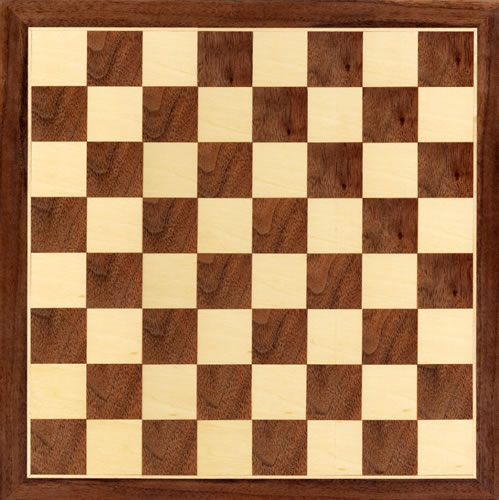
\includegraphics
 [scale=0.477,viewport=-20 17 -20 17]
 {brett}%
\chessboard[showmover=false,
            border=false,
            label=false,
            boardfontencoding=LSBC5,
            boardfontsize=20pt,
            whitepiececolor=brown!70,
            blackpiececolor=black,
            setfontcolors]
\end{LTXexample}

\subsection{Using the commands of \skaksty}

When used with the option \textsf{ps} \skaksty puts in the middle of
the right bottom field (that is either h1 or a8) a postscript node
with the name BM. The highlighting commands of \skaksty use this
node.

To be able to use the commands also with \cs{chessboard} you must
load \skaksty with the option \textsf{ps}.

As arguments in the commands of \skaksty you can only use the fields
of a 8\texttimes8-board.

\medskip
\Describesetkey{psset}{true|false}{}{false}

This key sets the  node BM at the place where \skaksty expect it,
\emph{and it sets the psunits to the size of the board}. This can
affect other pspictures as the changes are made after the board and
so aren't local to the board (the commands of \skaksty must have a
fighting chance to get the correct values).

\medskip
\Describesetkey{psskak}{true|false}{}{false}

This key redefines some internal commands of \skaksty. I had to do it
in order to get the highlighting commands to work. I don't think that
it will destroy anything but didn't want to activate the changes
unasked. The changes are also \emph{not} local to the board (but
local to the group).

\begin{LTXexample}[graphic={chessboard-skakps}]
\documentclass[parskip]{scrartcl}
\usepackage[T1]{fontenc}
\usepackage[ps]{skak}
\usepackage{chessboard}

\pagestyle{empty}
\begin{document}
\newchessgame
\chessboard[psskak,psset,pgf=false,
            inverse]
\ifpdf\else
\highlight[X]{c4}
\highlight[o]{a8}
\highlight[O]{g1}
\printknightmove{g8}{f6}
BM\pnode{A}\ncline{->}{A}{BM}
\fi
\end{document}
\end{LTXexample}





\subsection{Intelligent highlighting}

\cs{chessboard} doesn't know anything about chess rules. It can't do
things like «show me the possible moves of the rock», «show me the
allowed moves» or «highlight the last move». But as the examples show
it accepts commands as arguments in the highlighting keys, so it can
use the intelligence of external commands or applications. E.g.\
highlighting of the last move would be easy if \skaksty would somehow
save the last from-field and the last to-field -- something it
doesn't do now.

\section{Extending the game}
\subsection{Adding new pieces}
\DescribeMacro{\cbDefineNewPiece}
With this command you can add new pieces that can be used on the
board.

\cs{cbDefineNewPiece}\oarg{game}\marg{color}\marg{char}\marg{on
white}\marg{on black}

The optional argument \meta{game} has not much use yet as there is
only one sensible value \texttt{skak} which is the default anyway.
So leave it out.

\meta{color} should by either \texttt{white} or \texttt{black}, it
will put the character in the list used by e.g.\ the key
\key{hidewhite}.

\meta{char} is the character used in FEN and the other input
arguments. Use a uppercase char for white pieces and a lowercase
char for the black pieces or the keys like \key{addwhite} won't work
correctly.

\meta{on white} and \meta{on black} should contain the commands
needed to print the piece on white and black fields. The symbols
should be scalable. So you should either use symbols from a font or
use some resizing command from the graphicx package.

\begingroup
\begin{LTXexample}[width=0.25\textwidth]
\makeatletter
\cbDefineNewPiece{white}{C}
  {\raisebox{\depth}{\cfss@whitepiececolor
    $\heartsuit$}}
  {\BlackEmptySquare%
   \makebox[0pt][r]{\cfss@whitepiececolor
    \raisebox{\depth}{%
     \makebox[1em]{$\heartsuit$}}}}
\cbDefineNewPiece{black}{c}
  {\raisebox{\depth}{\cfss@blackpiececolor
    $\clubsuit$}}
  {\BlackEmptySquare%
   \makebox[0pt][r]{\cfss@blackpiececolor
    \raisebox{\depth}{%
     \makebox[1em]{$\clubsuit$}}}}
\makeatother
\setchessboard{tinyboard,
  addpieces={cd4,Ce5},addwhite={ca1,Cb1},
  addblack={ca8,Cb8}}
\chessboard[addpieces={cd4,Ce5, Ke4}]
\chessboard[hidewhite]
\chessboard[boardfontencoding=LSB3,
  whitepiececolor=red,blackpiececolor=blue,
  setfontcolors,color=lightgray,
  trimtocolor=black, colorbackboard]
\end{LTXexample}
\endgroup

%\subsection{Clipping and trimming the picture}



\subsection{Using \texorpdfstring{\cs{chessboard}}{\textbackslash chessboard} for other games}

I have tried to prepare \cs{chessboard} for other games. A lot of
internal commands can be changed simply by changing the «name of the
game». Up to now there isn't another game, so I don't know if this
will really work.


It should be easy to make boards for checkers if I find a font
somewhere. Chinese chess is a bit more complicated as one would have
to decide how to make the background lines. Go is more complicated
as the pieces are sometimes numbered, I don't know yet if I could
implement a good input handling -- but as there is a quite good
package named igo I don't think I will really look into it.


The main problem in any cases is the missing partner: \Pchessboard
isn't «intelligent». As already mentioned above it doesn't know
anything about the rules of chess. To be able to show «the running
game» it needs a partner that does the calculation.



\section{Compability with other packages}

\subsection{\packagename{skak}}
\Pchessboard works fine with \skaksty. You can use \cs{chessboard}
everywhere instead of \cs{showboard} etc.

\subsection{\packagename{texmate}}

The new \packagename{texmate} version use \skaksty to follow the
game. There is no problem to use \cs{chessboard} where the manual
suggest \cs{showboard}.  \packagename{texmate} also defines its own
diagram commands. They use internaly \cs{showboard}. I haven't made
much tests until now, but it looks like after a simple
\lstinline+\let\showboard\chessboard+ you can use \cs{chessboard}
instead. The main problem is that you can't use the argument of
\cs{chessboard}. You will have to set the board properties with
\cs{setchessboard}.


\subsection{\packagename{beamer}}

I wouldn't have thought it, but I had no problem to use
\cs{chessboard} with \packagename{beamer}.

The following listing shows an example. If your pdf-reader can handle
annotations you can see the result in the attached file:
\attachfile{chessboard_and_beamer.pdf}

\begin{lstlisting}
\documentclass{beamer}
\usepackage[T1]{fontenc}
\usepackage{chessboard, skak}
\begin{document}

\begin{frame}
\newchessgame
\only<1->{\setchessboard{hideall,showmover=false}}
\only<2->{\setchessboard{showpieces={p,P}}}
\only<3->{\setchessboard{showpieces={K,k}}}
\only<4->{\setchessboard{showpieces={Q,q}}}
\only<5->{\setchessboard{showpieces={R,r}}}
\only<6->{\setchessboard{showpieces={B,b}}}
\only<7->{\setchessboard{showpieces={N,n}}}
\chessboard
\end{frame}

\begin{frame}
\newchessgame\setchessboard{markstyle=border,color=blue}
\only<1>{\mainline{1.e4}}
\only<1>{\setchessboard{markfields=e4}}
\only<2>{\hidemoves{1.e4}\mainline{1... e5}}
\only<2>{\setchessboard{markfields=e5}}
\only<3>{\hidemoves{1.e4 e5}\mainline{2. Nf3}}
\only<3>{\setchessboard{markfields=f3}}
\only<4>{\hidemoves{1.e4 e5 2.Nf3}\mainline{2... Nc6}}
\only<4>{\setchessboard{markfields=c6}}

\chessboard
\end{frame}
\end{document}
\end{lstlisting}

\subsection{animate}

It also possible to use animate to get «moving» boards (you need a
recent pdf-viewer to see the effect). But it is quite tiresome to
input all the moves. That's why I wrote the package
\packagename{xskak}. It offers a possibility to store all positions
of a game  with \skaksty and then to loop through them. For an
example please read the documentation of \packagename{xskak}. Here an
example of the more tiresome input:

\begin{LTXexample}
\newchessgame
\unitlength1pt
\newcommand\currentboard{%
 \begin{picture}(150,150)
 \put(10,10){\chessboard}
 \end{picture}}
\begin{animateinline}[autoplay,loop]{1}%
\currentboard
\newframe\hidemoves{1.e4}%
\currentboard
\newframe\hidemoves{1... e5}%
\currentboard
\newframe\hidemoves{2. Nf3}%
\currentboard
\newframe\hidemoves{2... Nc6}%
\currentboard
\newframe\hidemoves{3.Bb5}%
\currentboard
\newframe\hidemoves{3... a6}%
\currentboard
\end{animateinline}
\end{LTXexample}


\phantomsection
\makeatletter\def\index@prologue{\section*{Index}\addcontentsline{toc}{section}{Index}}\makeatother
\printindex
\end{document}

\end{document}
